\chapter{Experiments in live introspection}
\label{ch:experiments}

This chapter serves the purpose of showcasing the library and validating its
usefulness for actual deep learning research. While the ultimate goal is to have
a set of well-researched metrics in place which can be used live during
training, the way to acquire these metrics requires extensive analysis from many
experiments. Therefore, the goal of this work is to obtain such metrics, not
actually use them. This entails that the library is used primarily for easily
gathering all the data from the necessary experiments, and not for supervising
the actual training.

The chapter is divided between a reproduction part (see
\cref{sec:adam}) and an original research part (see
\cref{sec:detecting_learning_rate_proprocess} and
\cref{sec:detecting_layer_saturation}). In the former, experiments are conducted
for two popular variations of gradient descent are reproduced and extended with
the help of the library. The goal is to fact-check claims made by the authors
and validate said claims on more scenarios than are shown in the respective
publications. This will serve to show how \texttt{ikkuna} could have been
employed for this type of work. The second part will be concerned with employing
the library to investigate hypotheses for diagnosing roadblocks in the training
preprocess. Recall from \cref{sec:motivation} the multitude of hyperparameters
for a deep learning model and training regimen. In this work, we will concern
ourselves with the question of figuring out a good learning rate and when to
stop training layers to reduce computation time.

This thesis is not concerned with advancing the state of the art in
classification. Instead, toy problems are developed in order to prove or
disprove that the proposed metrics have the potential to be useful in guiding
the training. A more thorough evaluation of the results on realistic
architectures and problem sizes would require significantly more time and
computational resources and is left for future work.

\section{Review: Stochastic Gradient Descent}%
\label{sec:review_stochastic_gradient_descent}

In this section, we briefly survey the stochastic gradient descent algorithm.
This algorithm is used (in some variant) for virtually all practical deep
learning models. The name derives from the fact that the model parameters are
updated in the direction of the negative gradient, which is the high-dimensional
derivative of the scalar loss function with respect to the model parameters. It
is stochastic as it only uses a subset of the training data at every time step
and thus only approximates the true gradient which would have to be computed
over the entire dataset to be learned.

In standard stochastic gradient descent, a loss $J$ of some the
model parameters $\boldsymbol\theta$ (here, the layer weights) is computed over the training set of $m$
examples by forming the expectation over the sample loss $L$:

\begin{align}
    J(\boldsymbol\theta) &= \mathbb{E}_{\mathbf{x},y\sim\hat{p}_{\text{data}}} L(\mathbf{x}, y, \boldsymbol\theta) \\
                         &= \frac{1}{m}\sum_{i=1}^{m}L(x^{(i)}, y^{(i)}, \boldsymbol\theta)
\end{align}
The cumulative loss can then be derived for $\boldsymbol\theta$

\begin{align}
    \nabla_{\boldsymbol\theta}J &= \frac{1}{m}\sum_{i=1}^{m}\nabla_{\boldsymbol\theta}L(x^{(i)}, y^{(i)}, \boldsymbol\theta)
\end{align}
per the sum rule of differentiation. The simplest form of parameter update rule
is then

\begin{align}
    \boldsymbol\theta &\leftarrow \boldsymbol\theta - \eta \nabla_{\boldsymbol\theta}J
\end{align}
with the learning rate $\eta$. There is no hard and fast rule on what this
parameter should be, and it is subject of large swathes of literature. Popular
modifications to the vanilla update rule are the use of momentum
\citep{jacobs1988increased}, per-layer learning rates (ibd.), reducing the rate
throughout training, or adapting the
learning rate based on mean and variance of gradients across past time steps
\citep{kingma2014adam}. Nevertheless, most of the time, training begins with an
arbitrarily chosen small learning rate around $0.001$ which is then adapted
either by the aforementioned mechanisms or by search over the parameter space on
a subset of the training data when computationally feasible.

\section{Experimental Methodology}%
\label{sec:experimental_methodology}

For all experiments, \texttt{ikkuna} is used for recording various metrics
during training without having to adapt to any specific model. Experiments are
run on a Google Cloud virtual instance with between $4$ and $8$ Intel Xeon CPUs
and $1$ to $2$  Nvidia Tesla K80 graphics cards with $11$ GB of video memory. The
information captured by \texttt{ikkuna} during training is logged to a MongoDB
schemaless database with the help of the \texttt{sacred} library. The data can
then be analysed off-line with MongoDB's Python interface. Plots are created
with \texttt{matplotlib}. % and \texttt{seaborn}.

\section{Detecting Learning Rate Problems}%
\label{sec:detecting_learning_rate_problems}

\subsection{State of the Art and Related Work}%

\subsection{Ratio-Adaptive Learning Rate Scheduling}%
\label{sub:ratio_adaptive_learning_rate_scheduling}

The first problem to be investigated is that of choosing an appropriate learning
rated. We begin with a brief review of gradient descent and then evaluate how
the update-to-weight ratio of model weights can be used to identify bad learning
rates or automate learning rate selection.

As a first hypothesis, we investigate a claim made by \citet{karpathycs231n} who
states that the ratio between updates and weights is a quantity which should be
monitored and constrained. He suggests a target of $\frac{1}{t} = 10^{-3}$ as a
reasonable value, but to the author's knowledge there has never been a thorough
investigation of this hypothesis. Because of this lack of exploration and the
celebrity of the proponent, this merits further investigation.

It seems intuitive that this target cannot be static throughout training, since
we usually decay the learning rate towards the end, leading to smaller magnitude
of updates (this is a prerequisite for theoretical convergence guarantees for
SGD, see \citet[p. 20]{saad1998online}). As a matter of fact, this can be easily
verified by running training with an update rule that scales each gradient so
that the update hits the target (the network does learn, but to a significantly
smaller final accuracy; see \cref{fig:fixed-ratio-opt}). It is also not clear
whether the target should apply to all layers equally, since this would
constitute a strong regulariser on the network parameters, limiting
expressiveness of the model. For instance, in networks with the (now outdated)
$\text{tanh}$ activation function, the later layer's gradients are larger as
fewer backpropagation steps have been done to them, and for this activation
function at least, each application of the chain rule entails multiplication
with a factor $< 1$ (as the tanh derivative never exceeds $1$ and decreases to
almost $0$ in both limits), so gradients become exponentially small. In fact,
the vanishing gradient problem was the main driver to introduce non-saturating
activation functions.  Other nonlinearites such as the rectified linear unit do
not exhibit the same behaviour, but that does not mean all layers must change at
the same rate.

\begin{figure}
    \centering
    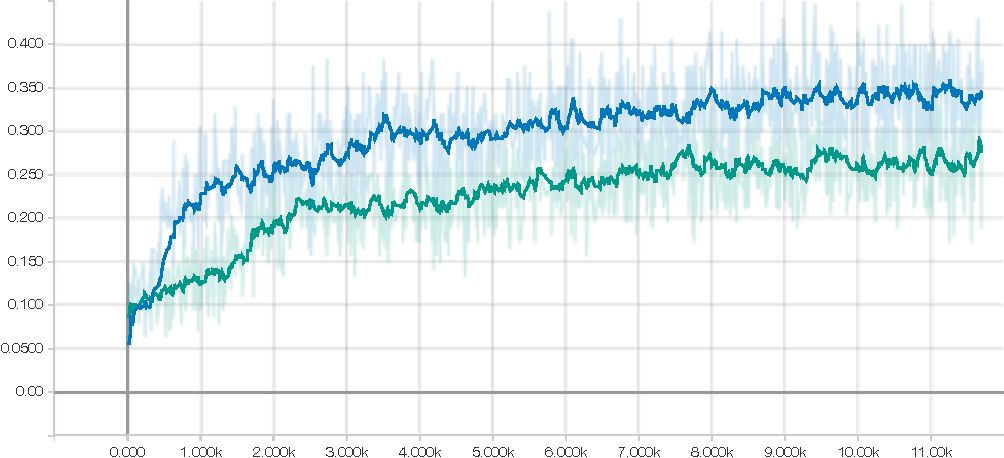
\includegraphics[width=\linewidth]{gfx/diagrams/experiments/ratio_loss_correlation/alexnetmini_sgd_fixed_ratio_01.pdf}
    \caption[Fixed-Ratio optimisation with AlexNetMini on CIFR10]{AlexNetMini on CIFAR10 at $0.1$ learning rate. The blue line is
    vanilla SGD while the green one is obtained by scaling the gradients to have
the updates meet a target ratio of $10^{-3}$}
    \label{fig:fixed-ratio-opt}
\end{figure}

As a first approach to an evaluation, we want to try and select the learning
rate in such a way as to hit the target postulated by
\citeauthor{karpathycs231n}, but not precisely for each layer, but on average
over all layers. This would allow for more flexibility in the weight updates
compared to fixing each update to the same value.

The experimental setup uses the simplified AlexNet architecture
(\cref{sec:pack-models}) shown in \cref{fig:alexnetmini}. The dataset used is
the well-known CIFAR-10 dataset consisting of $60.000$ $32\times32$ colour images
from ten object categories \citep{krizhevsky2009learning}. The optimisation
algorithm used is plain stochastic gradient descent on minibatches of size $128$. The
dataset does not constitute a hard problem to solve; state of the art accuracies
lie around $95\%$. For this reason, a decision must be made about how to make
the problem hard enough so that improvements to the training schedule can
actually be made. The learning rate has thus been fixed to a high value of $0.2$
which is not the optimal value (a learning rate of $0.1$ solves the problem to
$45\%$ accuracy).

\begin{figure}
    \centering
    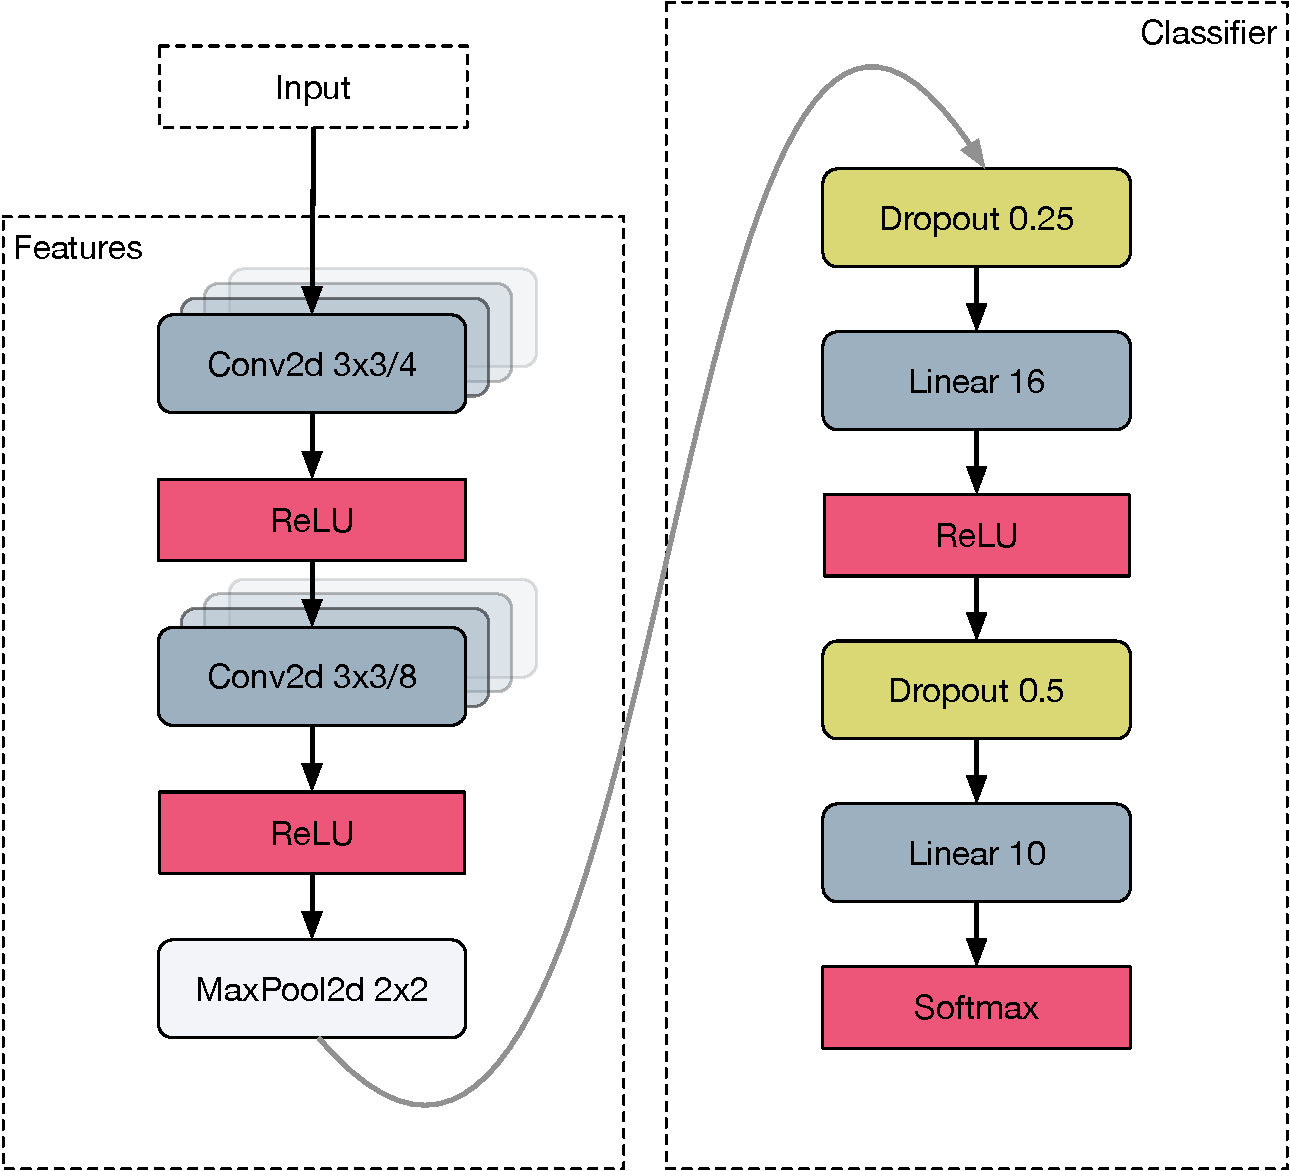
\includegraphics[width=\linewidth]{gfx/diagrams/neural_network/alexnetmini.pdf}
    \caption[Simplified AlexNet architecture]{The network used in this
    experiment. Image features are extracted by $4$ and $8$ convolutional
    filters, respectively, with ReLU nonlinearities. Maximum pooling is applied
    with a filter and stride size of $2$ leading to a resolution a fourth of the
    original size. The classifier portion employs dropout layers to reduce
    co-adaptation of units and a final softmax activation to map outputs to
    class probabilities in $(0,1)$.}
    \label{fig:alexnetmini}
\end{figure}

In order to validate that there is room for improvement (i.e.~the task is not
too easy), the training has been
run about twenty times for both a constant learning rate and an exponentially
decaying rate according to
\begin{equation}
    \eta_{e+1}  = 0.98^{e+1} \eta_{e},
\end{equation}
$e$ being the epoch index.
The final accuracies after $100$ epochs of training for constant learning rate,
exponential decay are shown in \cref{fig:validation1}. As can be seen, there is
a significant improvement when decaying the learning rate over keeping it
constant.

\begin{figure}
    \centering
    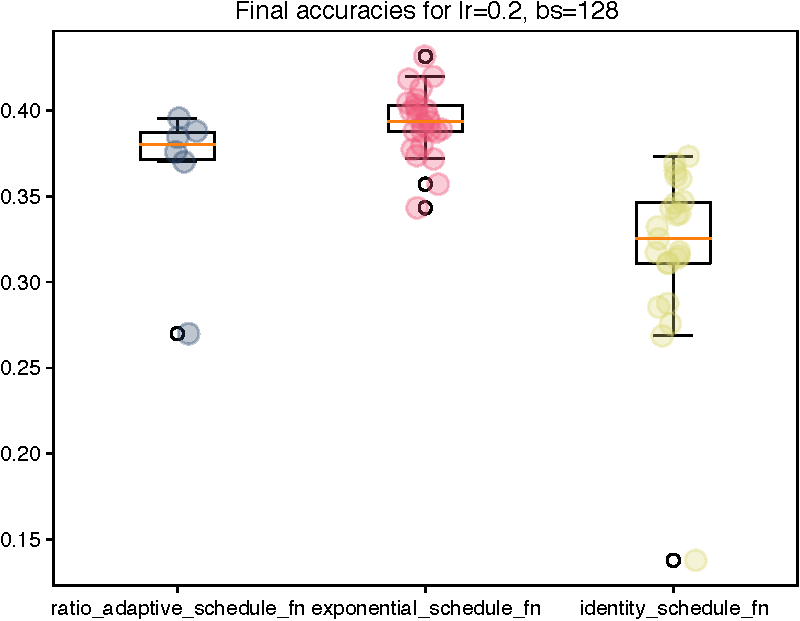
\includegraphics[width=\linewidth]{gfx/diagrams/experiments/experiment_validation.pdf}
    \caption[Final accuracies after 100 epochs]{Final accuracies after 100
    epochs with a learning rate of $0.2$ and batch size of $128$. The adaptive
    ratio schedule is discussed in\cref{sec:ratio-schedule}}
    \label{fig:validation1}
\end{figure}

\subsubsection{The Adaptive Update-to-Weight-Ratio Schedule}\label{sec:ratio-schedule}%

As a first showcase of the library and a test of the update-weight ratio
hypothesis, an adaptive learning rate based on the aforementioned ratio is
implemented with the help of the library.  We will start by formally describing
the update rule and then show how it is implemented with \texttt{ikkuna}.

Let $l$ be the number of layers with weight matrices associated with them (for
instance linear or convolutional layers, but not activation functions, dropout,
or the like). Let $\left\{W_{i,k} \mid i = 0 \ldots l - 1\right\}$ be the set of weight
matrices at training step $k$.  Let $\eta$ be the base learning rate and
$\frac{1}{t}$ be a target value to which we want the update-to-weigh ratio to
move. Furthermore, let $\gamma \in (0, 1)$ be a decay factor for exponential
smoothing.  Now, let

\begin{equation}
    R_{i,k} = \frac{||W_{i,k} - W_{i,k-1}||_2}{||W_{i,k}||_2}
\end{equation}
be the ratio between the $L2$-Norms of layer $i$'s weight updates before step $k$ step
and the weights at step $k$ themselves.  We then select the new learning rate
for batch step $k+1$ as

\begin{align}
    \eta_{k+1}   = \eta_{k}
                   \left(
                   t \cdot \frac{1}{l}
                   \sum_{i=0}^{l-1} \gamma R_k + (1 - \gamma) R_{k-1}
                   \right)^{-1}
\end{align}
for $k \ge 2$.  This is the average exponentially smoothed update-weight-ratio,
divided by the target range. This learning rate is used for vanilla gradient
descent without any other modifications beyond capping it to some value in case
of very small ratios. The effect of adapting the learning rate according to this
schedule is that the average ratio between the weight updates and the weights
moves towards the target range.  It should be noted that this update rule biases
the learning rate in favour of the smaller layers since all ratios are weighted
equally, regardless of the number of weights.
\cref{fig:schedule-accuracies} displays a set of accuracy traces for each of the
schedules (constant, exponential decay, ratio-adaptive) with different base
learning rates. The network was trained from scratch $5$ times for each combination.

\begin{figure}
    \centering
    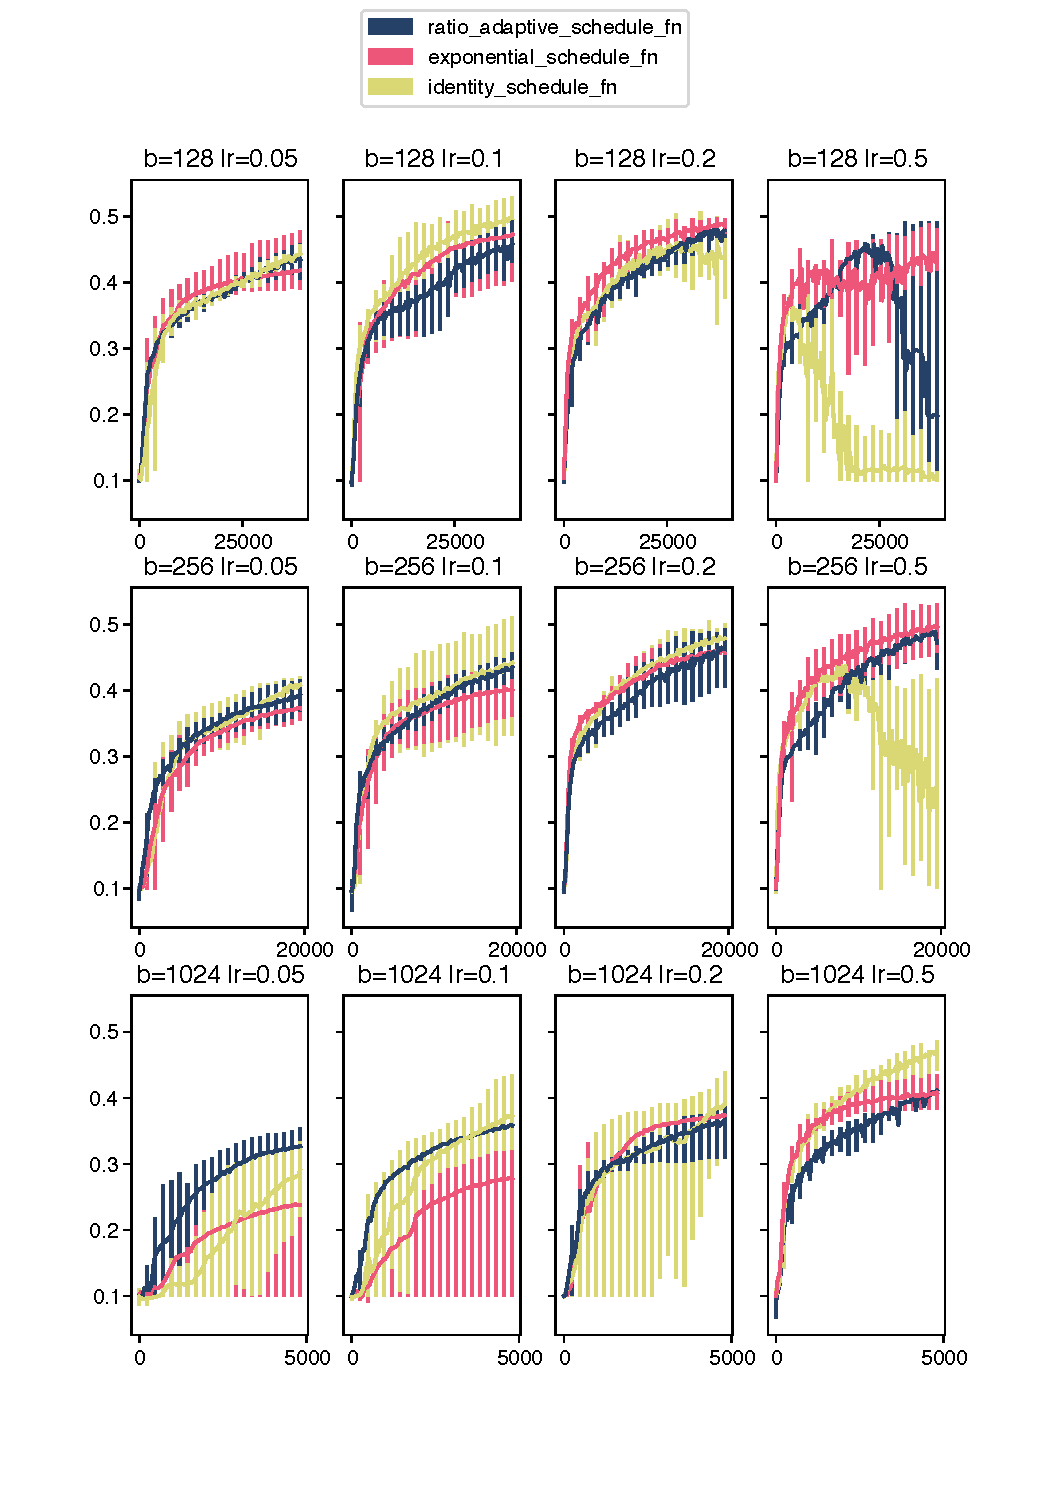
\includegraphics[width=\linewidth]{gfx/diagrams/experiments/ratio_adaptive_accuracies.pdf}
    \caption[Accuracy traces for different schedules on CIFAR-10]{Accuracy traces
    for different schedules on CIFAR-10. Batch size and initial learning rate are
    shown above each subplot. The exponential decay schedule uses a decay factor of
    $0.98$. Chance level is $0.1$. The experiments are run for $100$ epochs
    each.}
    \label{fig:schedule-accuracies}
\end{figure}

The results are not overwhelming, which is unsurprising for such a
simple schedule. For the smaller learning rates, it is not better or worse than
a constant or exponentially decaying schedule. However, for unnecessarily high
learning rates, the adaptive schedule outperforms the constant one, hinting at a
possible signal for identifying too high learning rates. This holds for the
smaller of the three batch sizes, which makes sense as a high batch size is
generally more amenable to a high learning rate, as the larger sample size
reduces the noise in the gradient and makes for a smoother loss landscape as the
gradients for more samples are averaged. On the other hand, the adaptive schedule
is also better than a constant one for very small learning rates on large batch
sizes. So it not only works in preventing too-high learning rates, but also too
low ones. This signal could hence be useful for
identifying inappropriate learning rates in small or large batch sizes.

As an impression of how the library presented in \cref{ikkuna} simplifies a
general implementation of such a learning rate schedule, code is provided here.

When an \verb+Exporter+ is configured for a given model, a
\verb+RatioSubscriber+ (see \cref{tbl:subscribers}) must be added to the message
bus in order for the update-weight-ratio ($R_{i,k}$ in the above equations) to be
published. One can then subscribe them and process the information with this
subscriber:
\begin{lstlisting}[language=Python]
class RatioLRSubscriber(PlotSubscriber):
    def __init__(self, base_lr, smoothing=0.9, target=1e-3, max_factor=500):
        subscription = Subscription(self, ['weight_updates_weights_ratio', 'batch_started'],
                                    tag=None, subsample=1)
        super().__init__([subscription], get_default_bus(),
                         {'title': 'learning_rate',
                          'ylabel': 'Adjusted learning rate',
                          'ylims': None,
                          'xlabel': 'Train step'})
        # exponential moving avg of R_{i,k}
        self._ratios     = defaultdict(float)
        # maximum multiplier for base learning rate (in pathological cases)
        self._max_factor = max_factor
        # exp smoothing factor
        self._smoothing  = smoothing
        # target ratio
        self._target     = target
        # this factor is always returned to the learning rate scheduler
        self._factor     = 1
        self._base_lr    = base_lr

    def _compute_lr_multiplier(self):
        '''Compute learning rate multiplicative. Will output 1 for the first batch since no layer
        ratios have been recorded yet. Will also output 1 if the average ratio is close to 0.
        Will clip the factor to some max limit'''

        n_layers = len(self._ratios)
        if n_layers == 0:   # before first batch
            return 1
        else:
            mean_ratio = sum(ratio for ratio in self._ratios.values()) / n_layers
            # prevent numerical issues and keep current LR in that case
            if mean_ratio <=  1e-9:
                return 1
            else:
                factor = self._target / mean_ratio
                return min(factor, self._max_factor)

    # invoked by the runtime for each incoming message
    def compute(self, message):
        if message.kind == 'weight_updates_weights_ratio':
            # the `key` property for these messages will be the module/layer
            # here we compute the exponential moving average of ratios
            i               = message.key
            R_ik            = message.data
            R_ik_1          = self._ratios[i]
            gamma           = self._smoothing
            self._ratios[i] = gamma * R_ik + (1 - gamma) * R_ik_1
        elif message-kind == 'batch_started':
            # before a batch starts, update the lr multiplier
            self._factor = self._compute_lr_multiplier()

    def __call__(self, epoch):
        return self._factor
\end{lstlisting}

The subscriber implements the \verb+__call__()+ method so it can be dropped into
PyTorch's learning rate scheduler (\verb+torch.optim.lr_scheduler.LambdaLR+).
This learning rate schedule can thus be used in every model, without modification.


\subsection{Effects Of Update-to-Weight-Ratio On Training Loss}%
\label{sub:effects_update_to_weight_ratio_on_training_loss}

We have seen in the previous section that at least for pathological cases the UW
ratio can be used to correct the learning rate to some extent. In this section,
we want to examine how this ratio does or should change during training. As
discussed in \cref{sub:ratio_adaptive_learning_rate_scheduling}, it is unlikely
that a constantly high rate of change to the weights will be beneficial
throughout the entire training. We would therefore like to find a relation
between the loss decrease, the current UW ratio and the point in time during
training. This could help us improve the learning rate schedule developed above
and refine the use of the UW ratio as a signal for inappropriate learning rates.

For this experiment, we learn CIFAR-10 for $75$ epochs, again with a batch size
of $128$, with vanilla SGD and the Adam optimizer and different learning rates.
We use the AlexNetMini architecture again, as well as a larger, more powerful
VGG network (schema in \cref{fig:vgg16}). We employ \verb+ikkuna+ to record
losses, accuracies and UW ratios for each layer automatically during training.
In order to make larger trends visible, we smooth the loss trace with a gaussian
kernel.

\begin{figure}
    \centering
    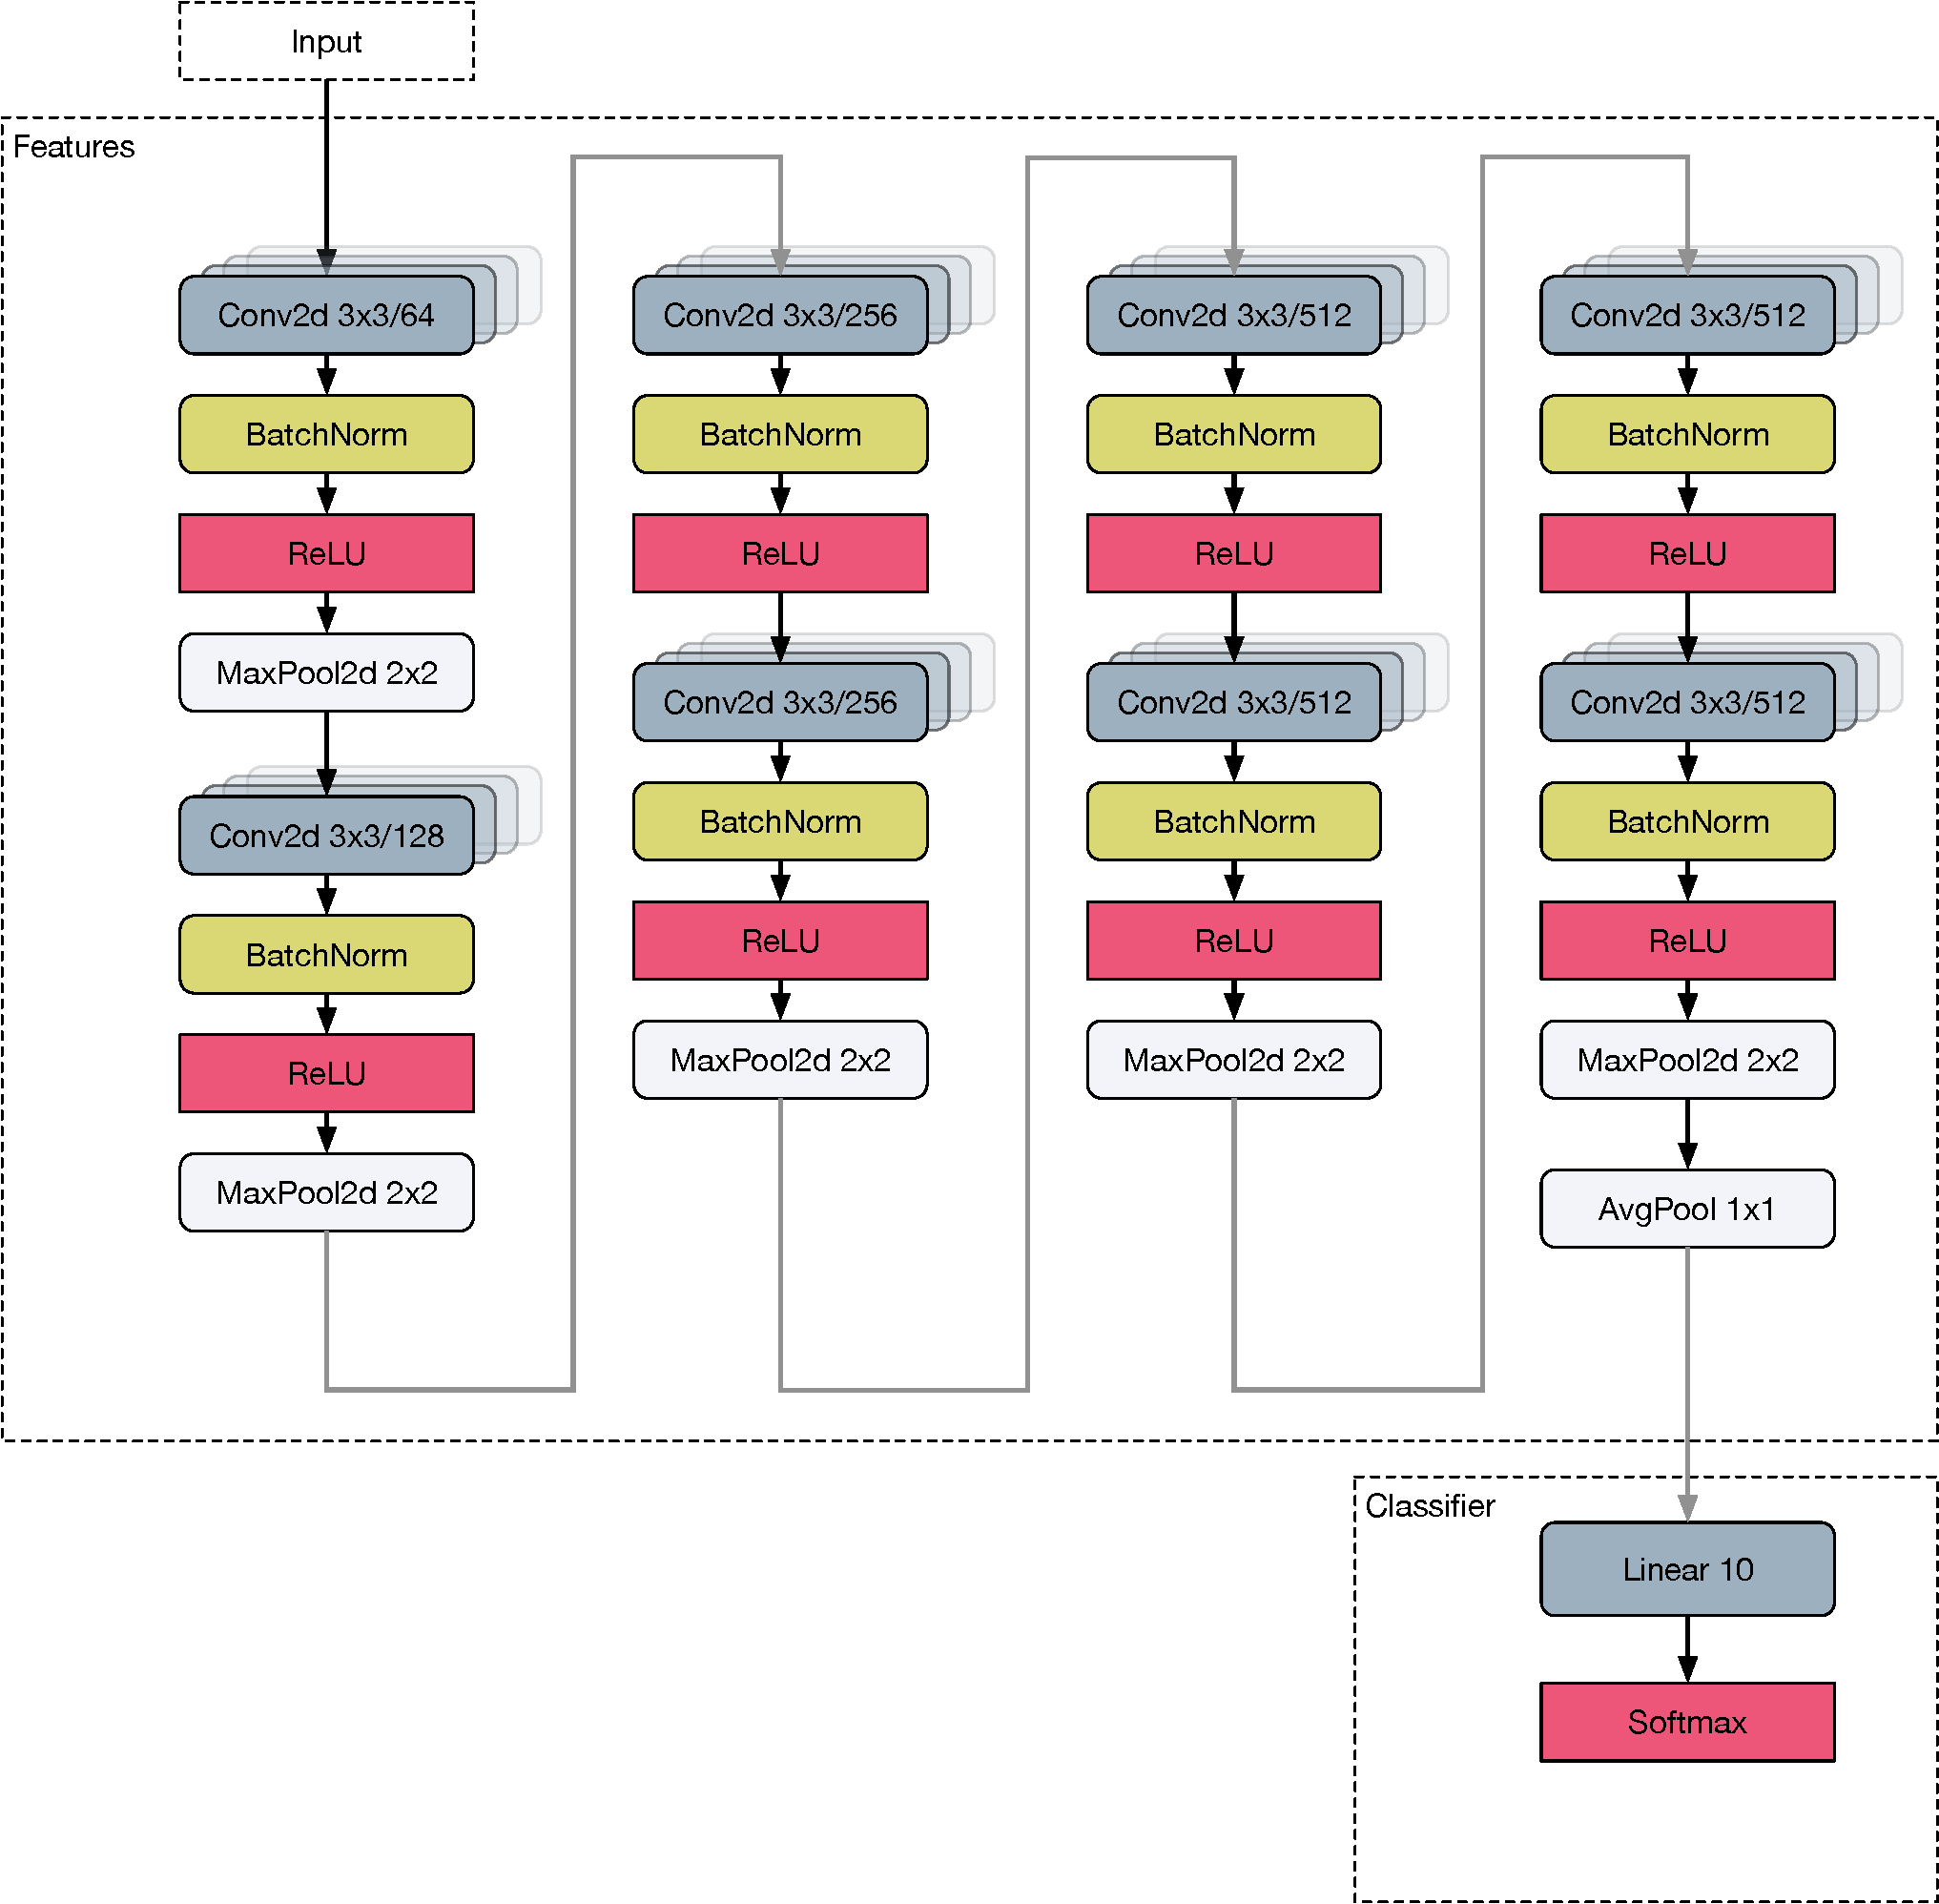
\includegraphics[width=\linewidth]{gfx/diagrams/neural_network/vgg.pdf}
    \caption[VGG network with $8$ convolutionsl layers.]{VGG network with $8$ convolutional layers.}
    \label{fig:vgg16}
\end{figure}

In the following figures, we plot the loss traces and their inverse derivative
(the amount of decrease) in the upper right, the average weight-update ratio in
the lower right, and a scatter plot of ratio versus loss decrease on the left.
The scatter plot has the time step colour-coded (blue is early, red is late) and
in addition offsets according to time on the $z$-axis. Due to the number of
points (up to $30.000$ time steps times the number of runs), the plots have been
subsampled where many points overlap. This was necessary to render the data for
this document. Care has been taken to not destroy the topology of the data.  The
density in a given area may thus not be entirely accurate. In the UW ratio
plots, the line displayed is the average over multiple runs.

\subsubsection{VGG with Stochastic Gradient Descent}

The plots in for this network only show the first $10.000$ training steps since
nothing of note happens afterwards. Since most of the ratio values cluster
around the same values towards the end of training, logarithmic subsampling was
applied.  For the VGG network, we observe a smooth decrease in the training loss
alongside a decrease in the average update-to-weight ratio. Training basically
stalls after around $10.000$ steps (about $25$ epochs).  We observe the trend
that the UW ratio is initially fairly high and falls off subsequently, which
correlates with a decrease in loss. However, there is no particular value of the
ratio that exhibits any significant correlations beyond other values. The
ratio in the beginning of training is also proportional to the learning rate, as
is to be expected.

It is curious that in the very beginning of training, the UW ratio has the
highest value, but the decrease in loss for these steps increases throughout the
first few batches (i.e. learning accelerates) before tapering off. This is
barely visible in the line plots, but shows as a prominent feature in the
scatter plot. It should be noted that this phenomenon happens on a very small
timescale -- the number of data points in the arc is orders of magnitude smaller
than in the rest of the plot, therefore it is no more than a curiosity. As a
preliminary conclusion, we can affirm that there is no linear correlation
between the ratio and the decrease in loss.

Furthermore, the smallest of the evaluated learning rates converges fastest.
The loss flatlines at $0$ after little more than $4000$ steps while the larger
learning rates need proportionally more time. The difference is marginal
however. The phenomenon might relate to the motivation for annealing the
learning rate: As we approach a local minimum, we need smaller learning rates to
not jump over it in a different direction in every update, but slowly fall into
the minimum itself. This may be an indication that an appropriate learning rate
for this particular problem is $\le 0.01$. None of the configurations exhibit UW
ratios close to Karpathy's suggestion of $10^{-3}$, but with the smallest
learning rate, we get closest, and converge fastest. Perhaps this could motivate
Karpathy's constant.

\begin{figure}
    \begin{subfigure}{\textwidth}
        \centering
        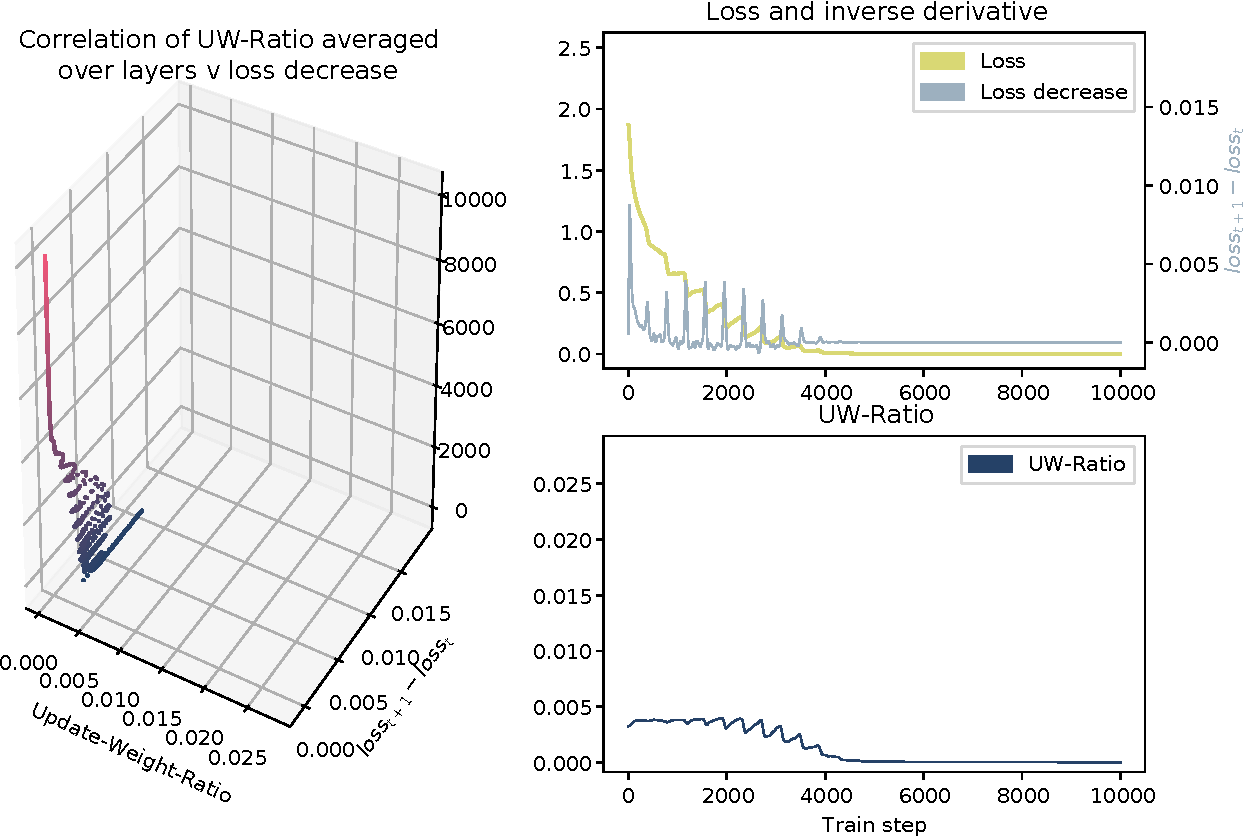
\includegraphics[width=\linewidth]{gfx/diagrams/experiments/ratio_loss_correlation/vgg_sgd_001_0_10000.pdf}
        \caption{UW ratio experiment for VGG with SGD and learning rate $0.01$}
        \label{fig:ratio_loss_corr_vgg_sgd_001}
    \end{subfigure}

    \begin{subfigure}{\textwidth}
        \centering
        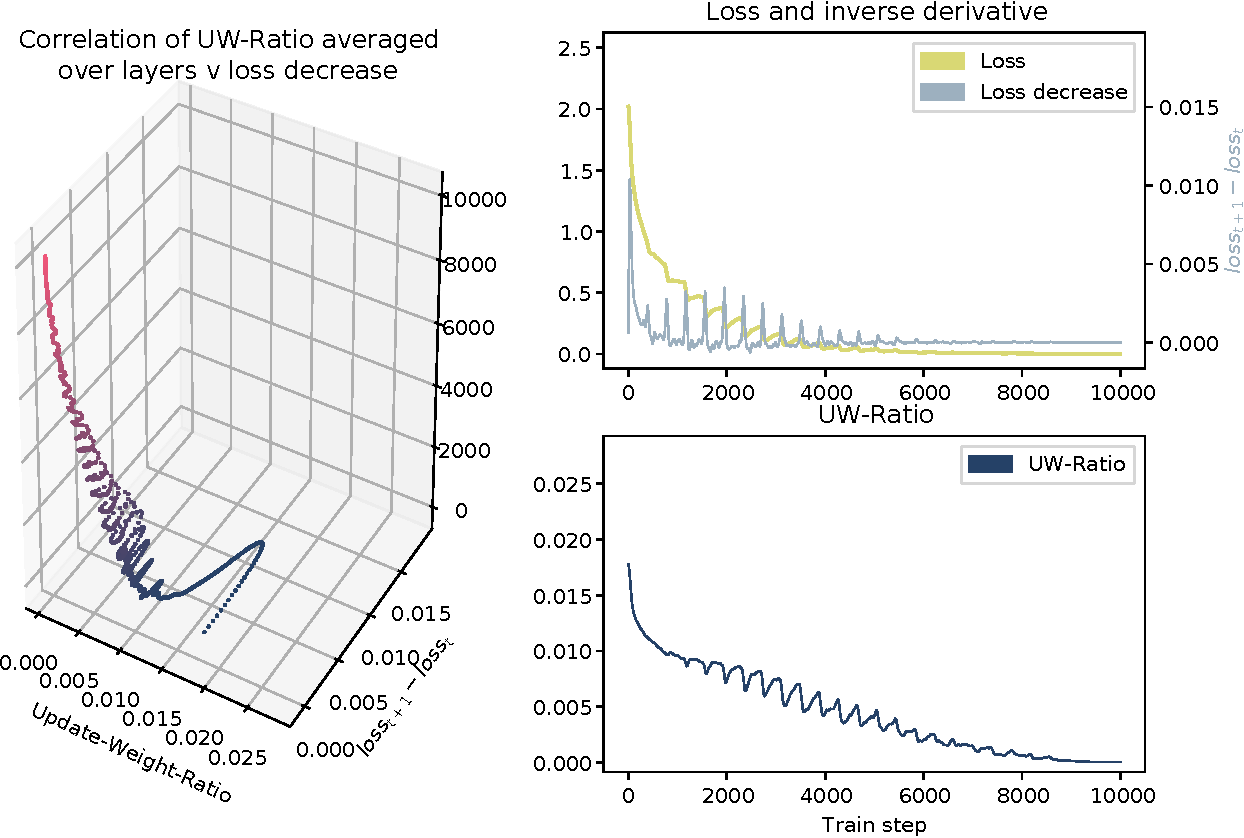
\includegraphics[width=\linewidth]{gfx/diagrams/experiments/ratio_loss_correlation/vgg_sgd_005_0_10000.pdf}
        \caption{UW ratio experiment for VGG with SGD and learning rate $0.05$}
        \label{fig:ratio_loss_corr_vgg_sgd_005}
    \end{subfigure}

    \begin{subfigure}{\textwidth}
        \centering
        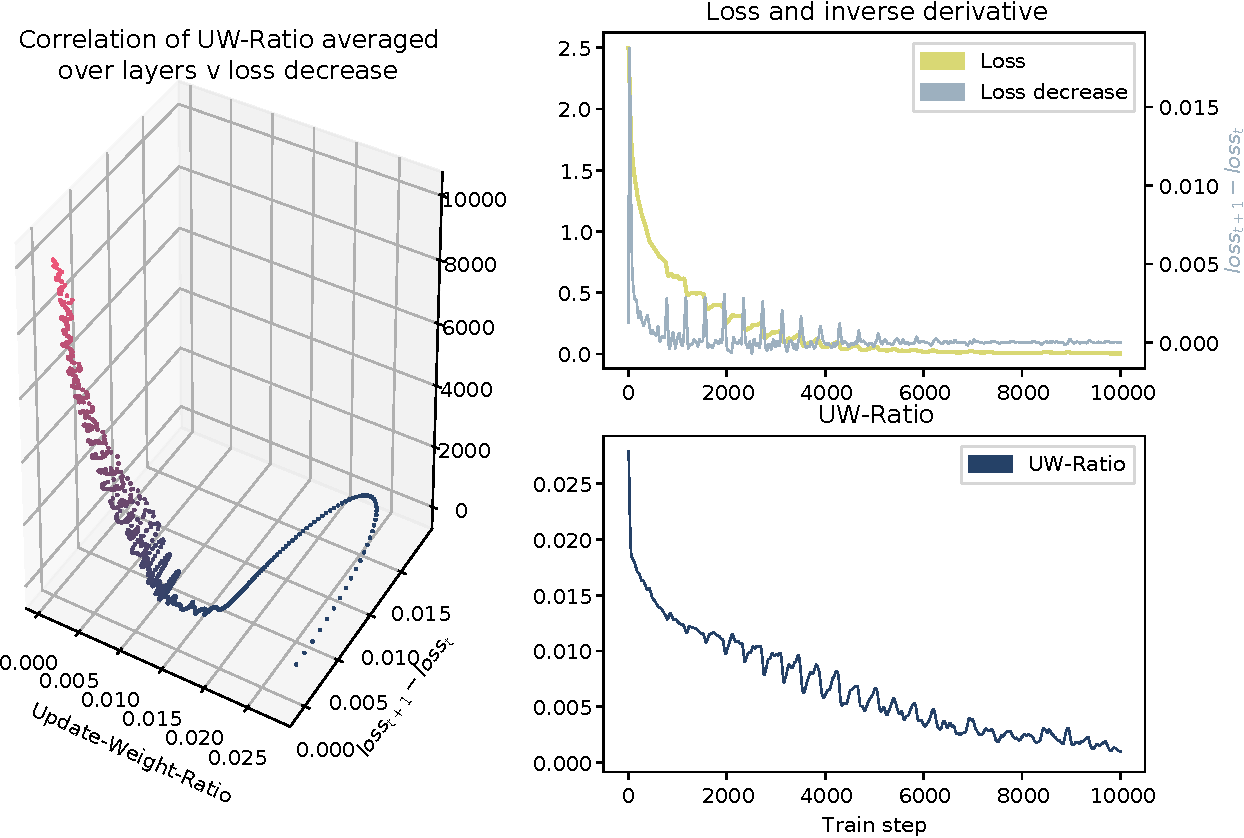
\includegraphics[width=\linewidth]{gfx/diagrams/experiments/ratio_loss_correlation/vgg_sgd_01_0_10000.pdf}
        \caption{UW ratio experiment for VGG with SGD and learning rate $0.1$}
        \label{fig:ratio_loss_corr_vgg_sgd_01}
    \end{subfigure}
\end{figure}

\subsubsection{VGG with Adam}

The same experiment has been run with the Adam optimizer \citep{kingma2014adam}
and has been found to produce quite different results. We mainly observe that
the steplike nature of the loss function (sharp decreases at epoch boundaries)
are much less pronounced with the Adam optimizer. This removes the loops  which we see for
SGD from the scatterplots. In absolute terms, Adam begets a much higher UW ratio
in the beginning of training, which falls off quickly to SGD's values.
Convergence takes minimally longer and doesn't occur at all with a learning rate
of $0.1$ (\cref{fig:ratio_loss_corr_vgg_adam_01}). Counterintuitively, the
adaptive optimiser is unable to adapt to the high learning rate and is
outperformed by vanilla SGD. The Adam optimiser keeps running estimates of the
mean and variance of the gradient of each parameter, with exponential smoothing
applied. The learning rate is adjusted for each parameter by multiplying it with
$\frac{\mu_{\text{grad}}}{\sqrt{\sigma_{\text{grad}}} + \epsilon}$. The argument
by \citet{kingma2014adam} is that in locations of high gradient variance, a
lower learning rate is appropriate since the estimate of the gradient at this
spot is noisy and unreliable, so smaller steps are a safer choice. Furthermore,
they claim that the mean of the gradient vanishes closer to an optimum, which is
also where we need to anneal the learning rate lest we jump over the minimum.
The Adam optimiser thus has learning rate annealing built-in. The step size
parameter $\eta$ is supposed to be of less importance since in Adam's parameter
update rule, it gives an upper bound on the size of the steps taken in parameter
space, but it can always be adjusted downward if the gradient variance is too
high. It can also be adjusted upward up to the upper bound if the gradient mean
is high, giving Adam momentum-like behaviour. The primary proposition of
\citet{kingma2014adam} is that manually tuning the learning rate per layer or
even per parameter is no longer necessary, but we see here that cases can be
found where precisely this behaviour of Adam would be needed -- we have set a
too-high learning rate, but Adam fails to compensate for this negligence. This
casts doubt on the universality of the Adam optimiser.\footnote{The hypothesis
that Adam starts to show its merit in the absence of batch normalisation could
not be tested on the VGG architecture, since training did not progress at all
with any learning rate or optimiser when batch normalisation layers were
removed. For the smaller AlexNetMini architecture with added batch
normalisation, Adam did not outperform SGD in the absence of batch norm. To the
contrary, Adam even lead to vanishing gradients when using batch normalisation.}

\begin{figure}
    \begin{subfigure}{\textwidth}
        \centering
        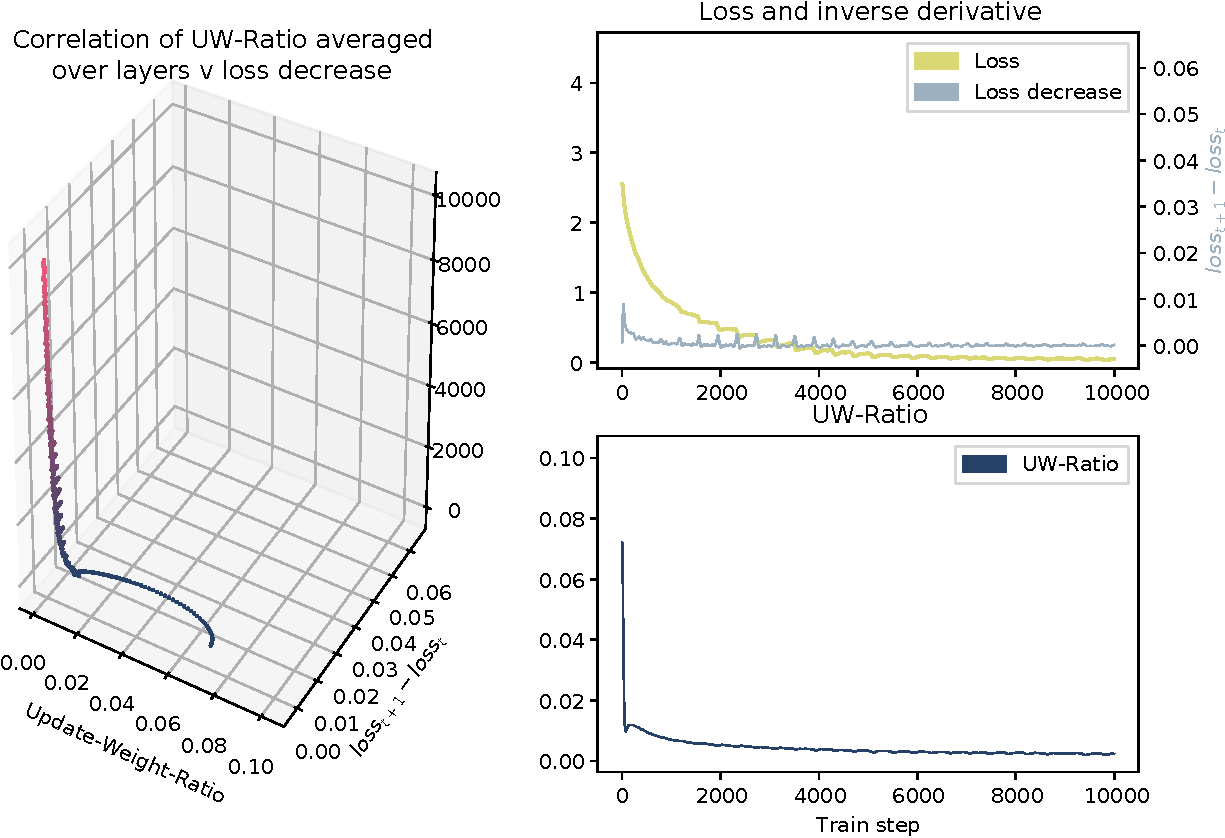
\includegraphics[width=\linewidth]{gfx/diagrams/experiments/ratio_loss_correlation/vgg_adam_001_0_10000.pdf}
        \caption{UW ratio experiment for VGG with Adam and learning rate $0.01$}
        \label{fig:ratio_loss_corr_vgg_adam_001}
    \end{subfigure}

    \begin{subfigure}{\textwidth}
        \centering
        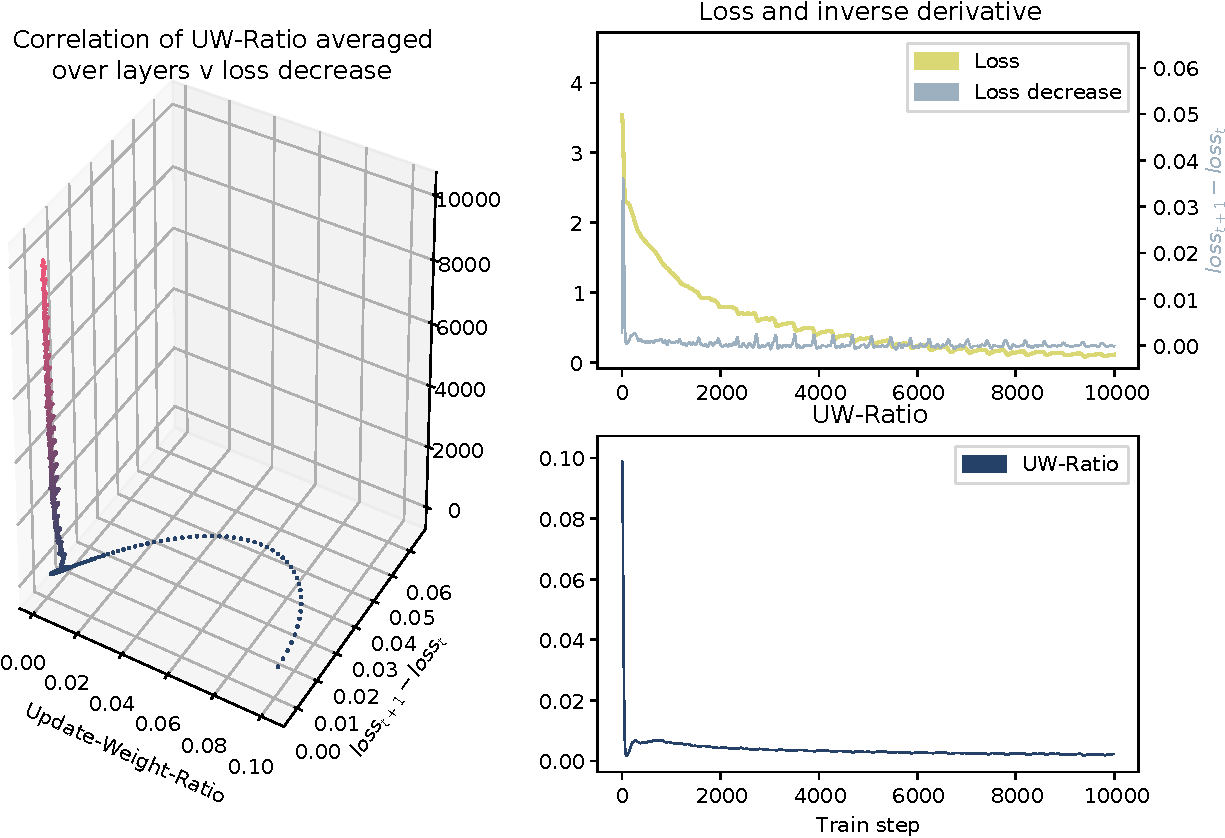
\includegraphics[width=\linewidth]{gfx/diagrams/experiments/ratio_loss_correlation/vgg_adam_005_0_10000.pdf}
        \caption{UW ratio experiment for VGG with Adam and learning rate $0.05$}
        \label{fig:ratio_loss_corr_vgg_adam_005}
    \end{subfigure}

    \begin{subfigure}{\textwidth}
        \centering
        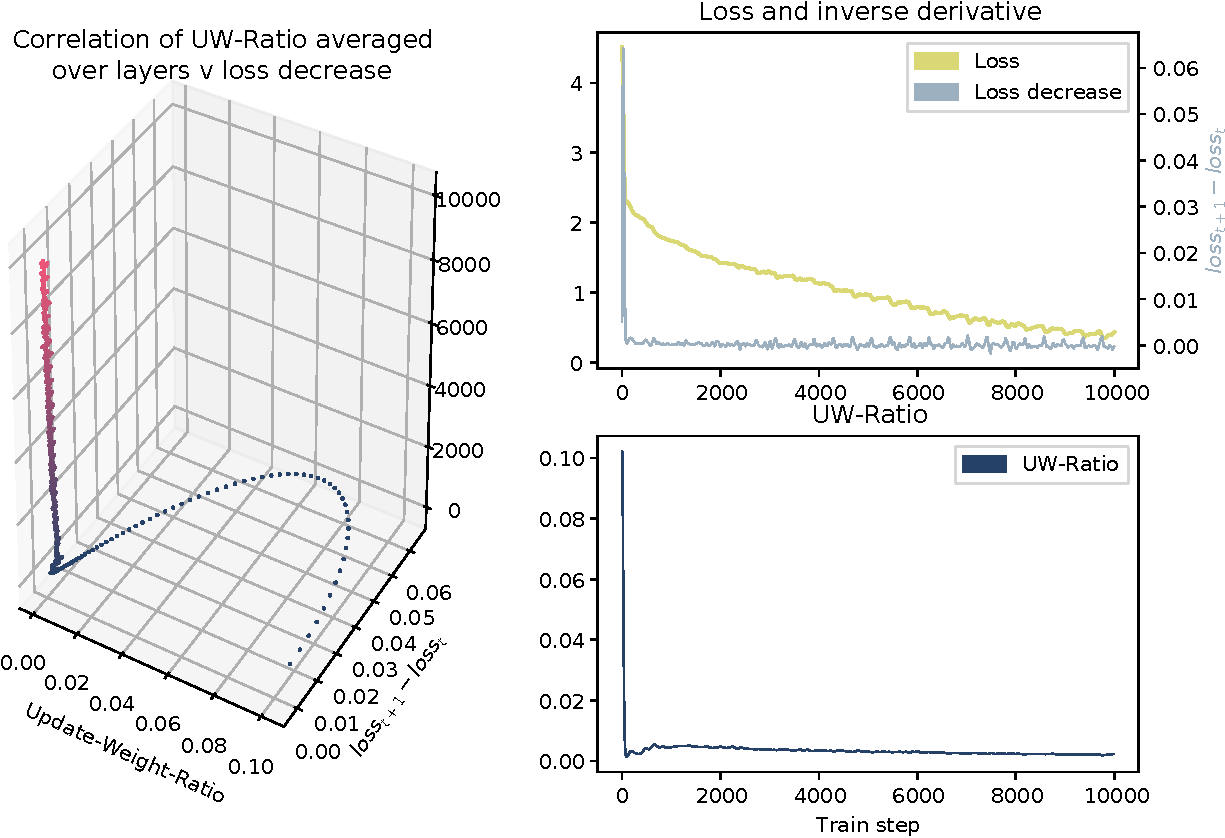
\includegraphics[width=\linewidth]{gfx/diagrams/experiments/ratio_loss_correlation/vgg_adam_01_0_10000.pdf}
        \caption{UW ratio experiment for VGG with Adam and learning rate $0.1$}
        \label{fig:ratio_loss_corr_vgg_adam_01}
    \end{subfigure}
\end{figure}

Remarkably, the qualitative behaviour is the opposite of SGD, which becomes visible
when omitting the first few hundred training steps. While for SGD (plots omitted
for brevity), higher learning rates lead to higher initial values in the UW
distribution, the opposite seems to hold for the adaptive optimizer. This can be
seen in
\cref{fig:ratio_loss_corr_vgg_adam_001_500,fig:ratio_loss_corr_vgg_adam_005_500,fig:ratio_loss_corr_vgg_adam_01_500}
where the first $500$ training steps are omitted to avoid squishing the
scatter plot because of the quickly decaying arcs in the beginning of training.
A possible explanation is that Adam uses estimates of the mean and variance of
gradients, and possibly overcorrects the learning rate.

\begin{figure}
    \begin{subfigure}{\textwidth}
        \centering
        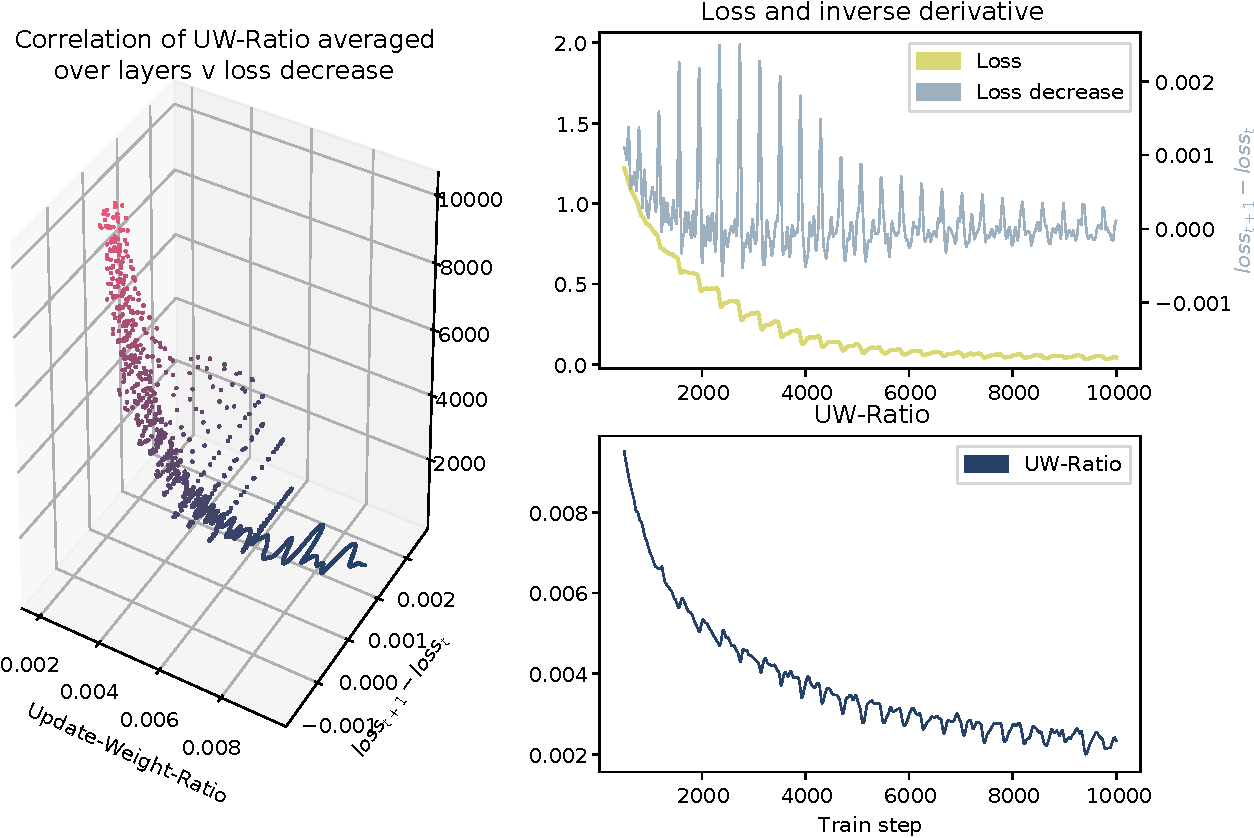
\includegraphics[width=\linewidth]{gfx/diagrams/experiments/ratio_loss_correlation/vgg_adam_001_500_10000.pdf}
        \caption{UW ratio experiment for VGG with Adam and learning rate $0.01$,
        beginning at step $500$}
        \label{fig:ratio_loss_corr_vgg_adam_001_500}
    \end{subfigure}

    \begin{subfigure}{\textwidth}
        \centering
        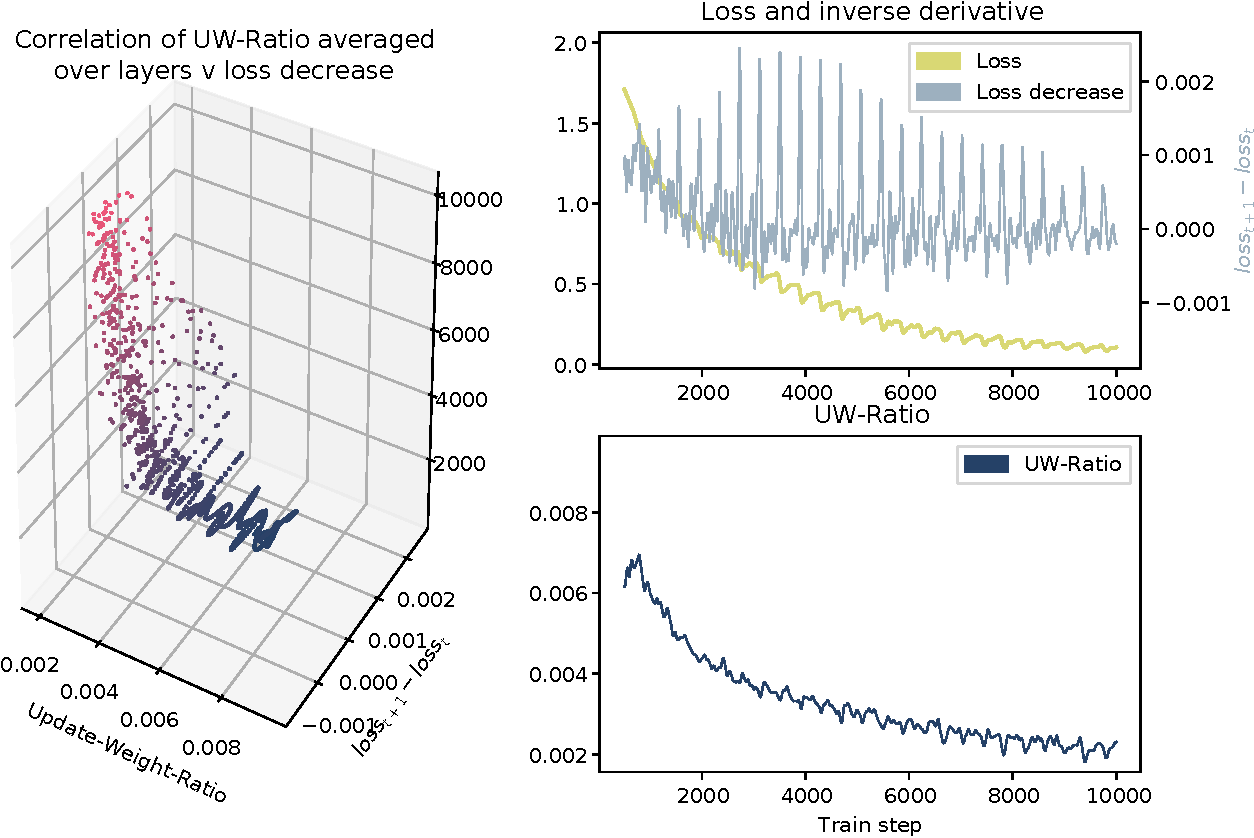
\includegraphics[width=\linewidth]{gfx/diagrams/experiments/ratio_loss_correlation/vgg_adam_005_500_10000.pdf}
        \caption{UW ratio experiment for VGG with Adam and learning rate $0.05$,
        beginning at step $500$}
        \label{fig:ratio_loss_corr_vgg_adam_005_500}
    \end{subfigure}

    \begin{subfigure}{\textwidth}
        \centering
        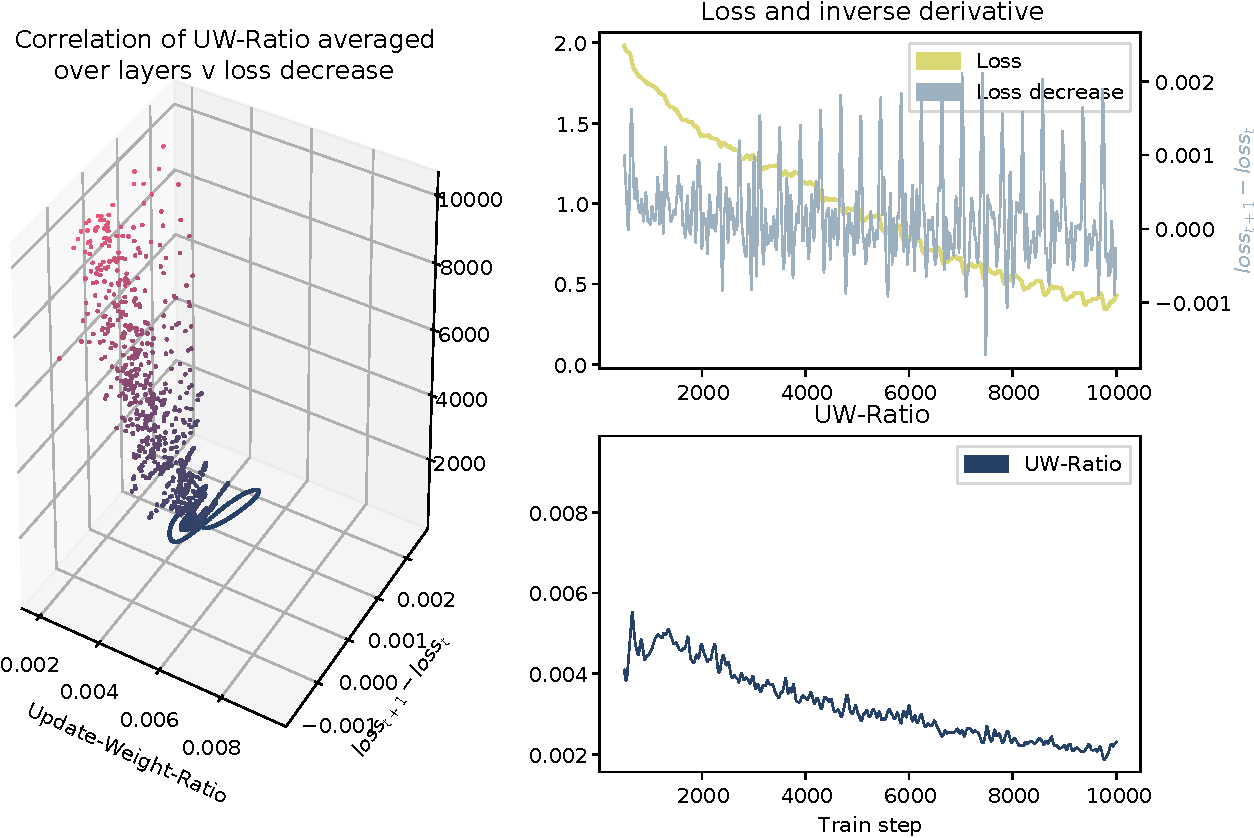
\includegraphics[width=\linewidth]{gfx/diagrams/experiments/ratio_loss_correlation/vgg_adam_01_500_10000.pdf}
        \caption{UW ratio experiment for VGG with Adam and learning rate $0.1$,
        beginning at step $500$}
        \label{fig:ratio_loss_corr_vgg_adam_01_500}
    \end{subfigure}
\end{figure}

\subsubsection{Other Architectures}

Several analyses were conducted on the data, but not displayed here due to
inconclusive results.
The experiments were run on the AlexNetMini architecture as well, without
results, as the network does not converge within $75$ epochs.
The same experiment on the ResNet18 architecture exhibited the same qualitative
behaviour as the VGG network, except for a larger variance in loss decreases for
a given ratio value. Slicing the training into pieces and graphing every slice
of $5000$ training steps separately reveals nothing beyond a decrease in
absolute value of ratio and loss, which is expected. Any correlations between
the two quantities do not change after the initial few steps.

\subsubsection{Conclusion}

The results from all these experiments do not demonstrate that a ratio value
of $0.001$ is any more significant than others. While it is intuitive that the loss
can only decrease significantly if the weights change accordingly (unless the
loss surface is extremely rough), we find no particular insights as to what
ratio is appropriate for any given point in training.

\subsubsection{Ratio-Adaptive Learning Rate Scheduling}

We now want to check how the UW ratio relates to the loss when we attempt to
artificially fix the ratio value to a target of $0.001$. Since the updates to the
weights in vanilla SGD (see \cref{sec:review_stochastic_gradient_descent}) are a
function of the learning rate and the gradient magnitude, this could be done in
one of two ways
\begin{enumerate}
    \item Scale the gradients with the constant learning rate in mind
    \item Set the learning rate according to the ratio-adaptive schedule from
        \cref{sub:ratio_adaptive_learning_rate_scheduling}
\end{enumerate}

Using the ratio-adaptive schedule results in the behaviour shown in
\cref{fig:ratio_loss_corr_vgg_sgd_0001_adaptive,fig:ratio_loss_corr_vgg_sgd_001_adaptive,fig:ratio_loss_corr_vgg_sgd_01_adaptive}.
In contrast to previous experiments, we also have a configuration with $0.001$
learning rate, dropping the $0.05$ value. We also plot the learning rate caused
by the scheduling over the UW ratio.

Note that for this set of plots, the axis limits are different. This serves to
illustrate that the qualitative behaviour is identical for all learning rates
(ignoring the fast arc at the beginning for $\text{lr}=0.1$). The learning rate
trajectories are very similar; the learning rate rises as the UW ratio
decreases. The primary insight from these experiments is that the empirical UW ratio is
not linearly related to the learning rate. Recall from
\cref{sec:review_stochastic_gradient_descent} that the weight update is given by
\begin{align}
    \eta \nabla_{\boldsymbol\theta}J,
\end{align}
so it is a linear function of the learning rate and the gradient magnitude. We
would therefore expect that a tenfold reduction in learning rate would result in
an equal reduction in the UW ratio. However, the difference is not quite as
pronounced in reality. Considering
\cref{fig:ratio_loss_corr_vgg_sgd_001_adaptive} and
\cref{fig:ratio_loss_corr_vgg_sgd_01_adaptive} we see the learning rate
differing by a factor of $\sim{}5$, whereas the UW ratios only differ by a factor of
$\sim{}2$. The cleft between reality and expectation is even more pronounced for
learning rates $0.001$ and $0.1$. This hints at a qualitative difference between
the paths through parameter space taken by higher vs. lower learning rates. If
we assume the directions are mostly the same, we would also expect the higher
learning rate to traverse them quicker (entailing a larger weight change and
thus a higher UW ratio, but possibly suffering from the usual problems of
too-high learning rate). If instead the path taken by the higher learning rate
is actually less steep than the one taken by the smaller rate, we could observe
the phenomenon documented here.

\begin{figure}
    \begin{subfigure}{\textwidth}
        \centering
        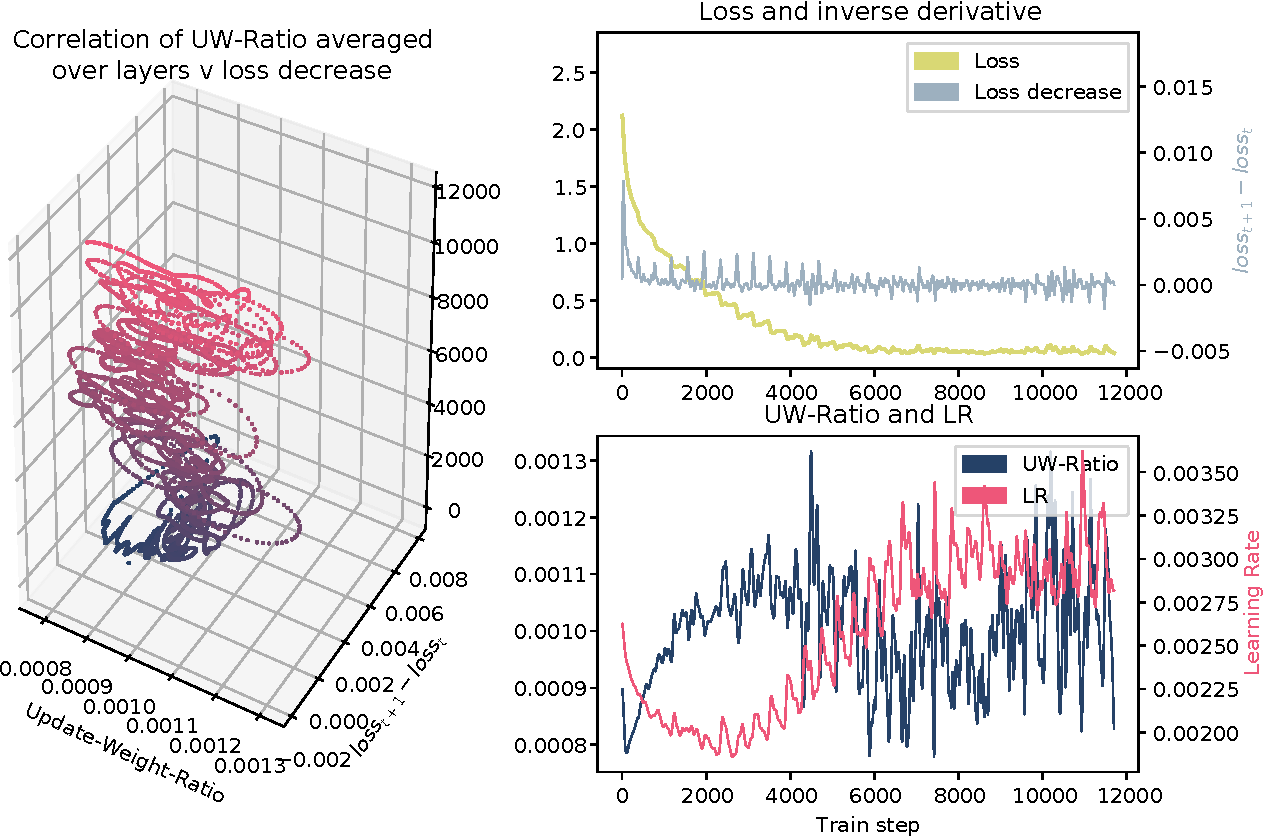
\includegraphics[width=\linewidth]{gfx/diagrams/experiments/ratio_loss_correlation/vgg_sgd_0001_0_11700_ratio_schedule.pdf}
        \caption{UW ratio experiment for VGG with SGD and adaptive learning rate
            from $0.001$}
        \label{fig:ratio_loss_corr_vgg_sgd_0001_adaptive}
    \end{subfigure}

    \begin{subfigure}{\textwidth}
        \centering
        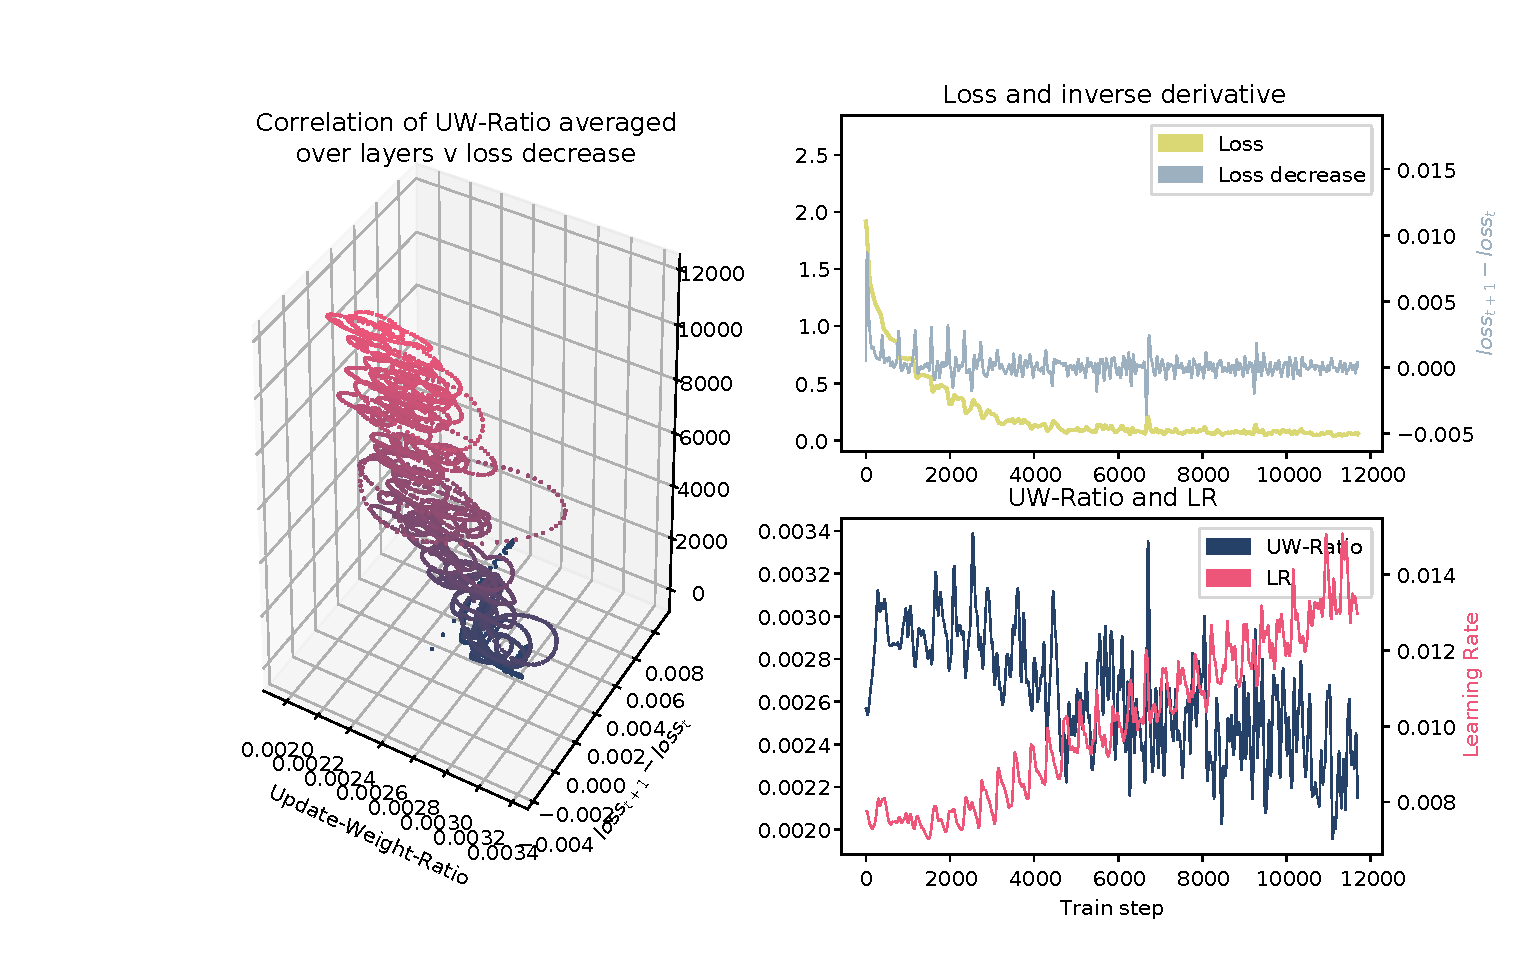
\includegraphics[width=\linewidth]{gfx/diagrams/experiments/ratio_loss_correlation/vgg_sgd_001_0_11700_ratio_schedule.pdf}
        \caption{UW ratio experiment for VGG with SGD and adaptive learning rate
            from $0.01$}
        \label{fig:ratio_loss_corr_vgg_sgd_001_adaptive}
    \end{subfigure}

    %% leave this as only 3 fit on one page
    % \begin{subfigure}{\textwidth}
    %     \centering
    %     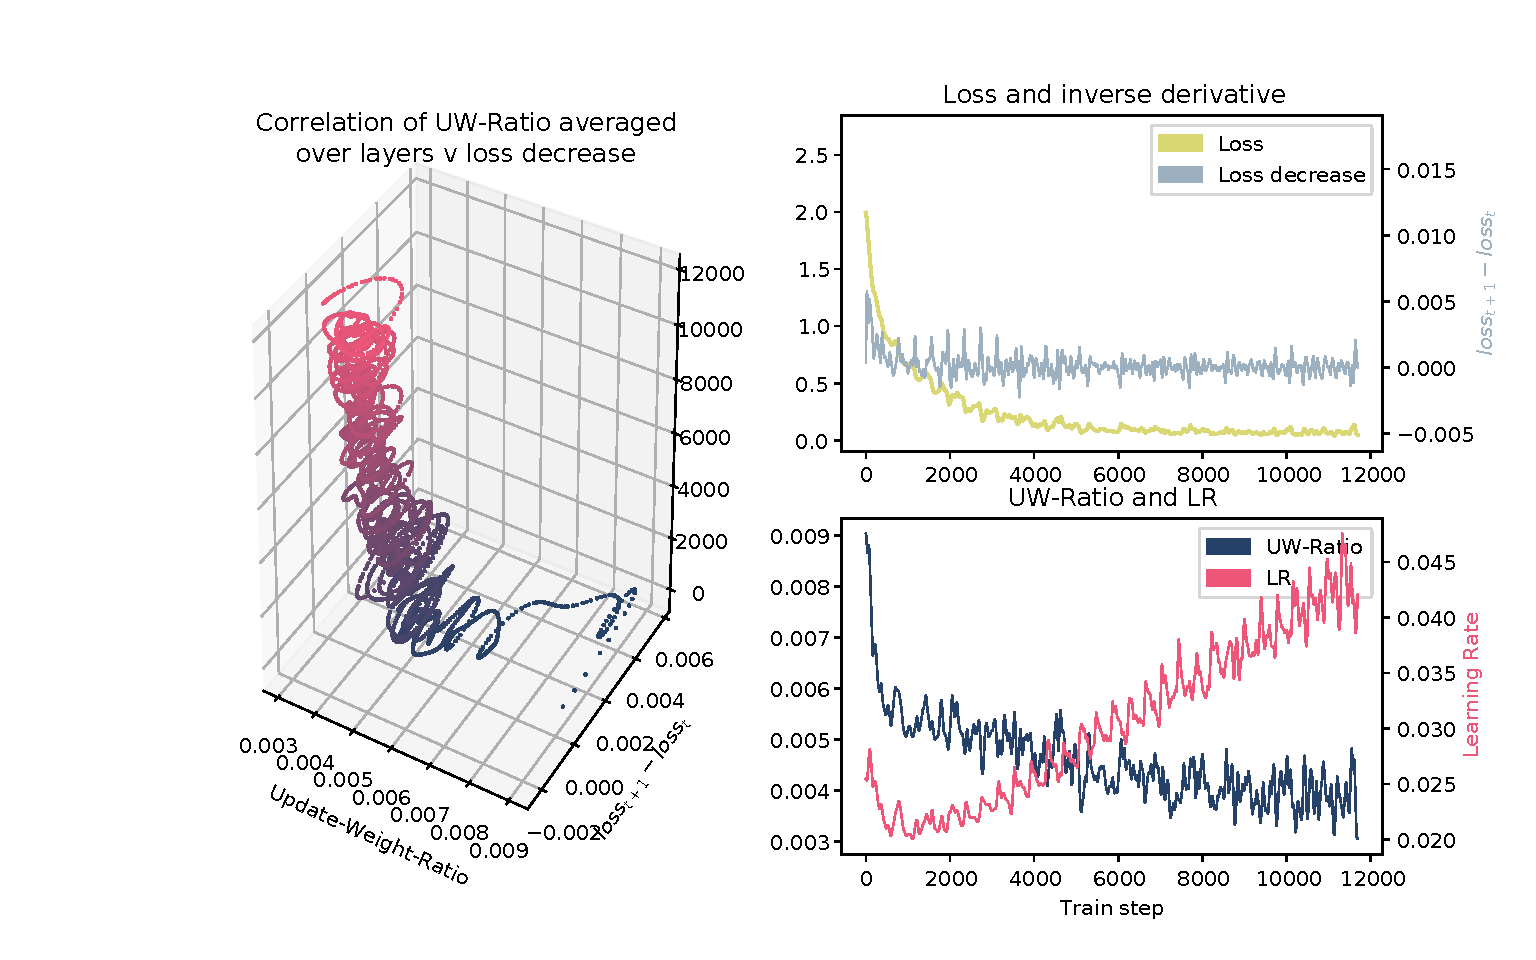
\includegraphics[width=\linewidth]{gfx/diagrams/experiments/ratio_loss_correlation/vgg_sgd_005_0_11700_ratio_schedule.pdf}
    %     \caption{UW ratio experiment for VGG with SGD and learning rate adaptive
    %         from $0.05$}
    %     \label{fig:ratio_loss_corr_vgg_sgd_005_adaptive}
    % \end{subfigure}

    \begin{subfigure}{\textwidth}
        \centering
        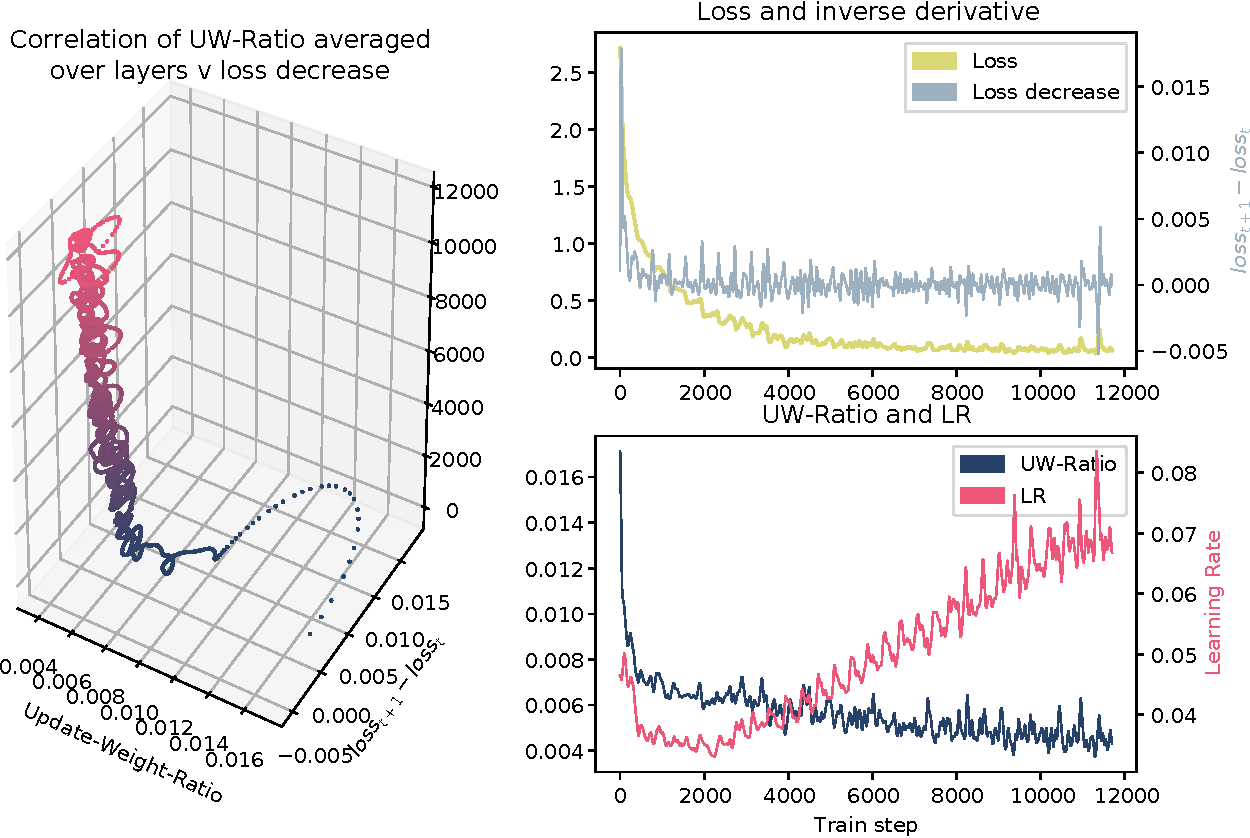
\includegraphics[width=\linewidth]{gfx/diagrams/experiments/ratio_loss_correlation/vgg_sgd_01_0_11700_ratio_schedule.pdf}
        \caption{UW ratio experiment for VGG with SGD and adaptive learning rate
            from $0.1$}
        \label{fig:ratio_loss_corr_vgg_sgd_01_adaptive}
    \end{subfigure}
\end{figure}

\subsubsection{Conclusion}

The two experiments with a dynamic learning rate schedule based on the average
ratio of updates and parameters do not yield any definitive insights into
whether any one value should be considered a target metric. It was obvious from
the beginning that as the loss curve approaches its asymptote, the change to the
weights needs to decrease, and indeed this has been demonstrated clearly. It is
not clear at this point whether the UW ratio provides additional information
over other metrics such as the loss curve itself or the norm of the gradients,
but the experiments in influencing the ratio have proven that there is no
obvious dependency between them -- problems can still be learned with a smooth
loss decrease even when influencing the UW ratio via learning rate scheduling.

However, more work would be necessary to check whether a moving target could
help optimisation. We have seen througout this section that  when learning works
well, the ratio decays similarly to a an exponential, which opens the
possibility for scheduling the learning rate with some decay function and a base
value (such as $10^{-3}$).  While this may not aid convergence in cases that are
well-behaved, it could move models out of areas they would otherwise spend too
much time in, or reduce parameter oscillations in the face of highly noisy loss
surfaces.

With the help of \texttt{ikkuna}, one could easily implement a ratio-based
learning rate schedule with e.g. exponential decay built-in an test its
performance on a wide range of models and datasets.

\section{Validating Optimiser Research}%
\label{sec:adam}

In this section, we want to highlight the \texttt{ikkuna}'s usefulness in
scientific research by conducting experiments in the context of
\citep{kingma2014adam} and investigating in how far the claims made therein hold
true on a range of problems. The work investigates the Adam optimisation
algorithm on several machine learning problems, notably learning a convolutional
network on the CIFAR10 dataset.

\subsection{The Adam update rule}%
\label{sub:the_adam_update_rule}

While standard SGD only makes use of the gradients in the current time step to
compute a parameter update, Adam keeps an exponential moving average of the
gradient ($m_t$) and its square ($v_t$), supposedly as an estimate for the mean
and variance of the gradient around the current point in parameter space. This
estimate is computed for each parameter, meaning Adam incurs a memory overhead
of $\mathcal{O}(d)$ where $d$ is the number of model parameters. Since the
estimates are initialised with zero, a bias correction (denoted by
$\widehat{\cdot}$) is applied.

The parameter updates are computed as
\begin{align*}
    \theta_t \leftarrow \theta_{t-1}  - \eta \frac{\widehat{m}_t}{\sqrt{\widehat{v}_t} +
    \epsilon}
    \label{eq:adam}
\end{align*}
\citeauthor{kingma2014adam} justify the rule like this:
\begin{quote}
    With a smaller SNR [quotient of mean and square root of variance] the
    effective stepsize $\Delta_t$ will be closer to zero. This is a desirable
    property, since a smaller SNR means that there is greater uncertainty about
    whether the direction of $m_t$ corresponds to the direction of the true
    gradient. For example, the SNR value typically becomes closer to $0$ towards
    an optimum, leading to smaller effective steps in parameter space: a form of
    automatic annealing.
\end{quote}

Intuitively, the magnitudes of the update to a parameter will scale linearly
with the manitude of the running gradient mean (which is effectively a form of
momentum), but normalised with the magnitude of the running gradient variance so
that the update is smaller when the gradient is very noisy and larger when there
is more certainty of the direction of the true gradient.

\subsubsection{The Role of \texttt{ikkuna}}%
\label{sub:use_of_ikkuna_for_optimiser_research}

We use the \texttt{ikkuna} library to compute and record various metrics during
reproduction and extension of \citeauthor{kingma2014adam}'s experiments. This
section showcases how little code is required to implement a recording setup
portable to any neural network model. A subscriber is employed to record
\begin{enumerate}
    \item The biased first moment estimate (exponential running gradient)
    \item The biased second moment estimate (exponential running squared
        gradient)
    \item The bias-corrected first moment estimate
    \item The bias-corrected second moment estimate
    \item The effective learning rate
\end{enumerate}

For all metrics, mean, variance, median, and norm are logged in some interval,
as computing the median incurs $\mathcal{O}(n\log n)$ runtime cost for each
layer. Since Adam doesn't directly use the current gradients for its parameter
updates, we need to extract the effective learning rate used for a layer
somehow. Since we have access to the gradient $\nabla_t(L)$ and the update
$\Delta_t$ in each train step, we can divide the two to obtain
$\frac{\Delta_t}{\nabla_t(L)}=\eta$ which is the learning rate we would need to use
in a vanilla SGD step with the current gradients. However, gradients can be zero
at any time, and the corresponding update may not be, since Adam uses
gradients from the previous steps as well. We thus simply ignore invalid values
through division by zero in computing the metrics. In the pathological case
where this leads to an empty tensor, we log $0$ for display purposes, since we
would otherwise have to work around metric logs with different step vectors.

The subscriber used for recording all the information is displayed in
\cref{lst:running_moments_sub}. A second subscriber is used to log all the
computed metrics to a MongoDB database via the \texttt{sacred} library. While
the cleaner approach here would be to implement a \texttt{SacredBackend} to log
the metrics automatically, this would require some thought about the differing
capabilities of different backends. For instance, there is no native form of
histogram storage in \texttt{sacred}, while it is easy to provide through
TensorBoard or Matplotlib. Therefore, this backend is left for future work and a
Subscriber ist used instead for this limited set of experiments.

\begin{lstlisting}[label={lst:running_moments_sub},
caption={Subscriber to record Adam terms}]
class BiasCorrectedMomentsSubscriber(PlotSubscriber):

  def __init__(self, lr, beta1, beta2, eps, message_bus=get_default_bus(), tag=None, subsample=40, ylims=None, backend='tb'):

    title        = 'gradient_moments'
    ylabel       = 'Gradient Moments'
    xlabel       = 'Train step'
    subscription = Subscription(self, ['weight_gradients'], tag, subsample)
    super().__init__([subscription], message_bus,
                     {'title': title,
                      'ylabel': ylabel,
                      'ylims': ylims,
                      'xlabel': xlabel},
                     backend=backend)

    # all parameters to Adam
    self._lr    = lr
    self._beta1 = beta1
    self._beta2 = beta2
    self._eps   = eps

    # records of the running moment estimates
    self._means = dict()
    self._vars  = dict()

    # here we set up all the metrics to be published
    for pub_name in {
      'biased_grad_mean_estimate_mean',
      'biased_grad_mean_estimate_median',
      'biased_grad_mean_estimate_var',
      'biased_grad_var_estimate_mean',
      'biased_grad_var_estimate_median',
      'biased_grad_var_estimate_var',
      'biased_grad_mean_estimate_norm',
      'biased_grad_var_estimate_norm',
      'grad_mean_estimate_mean',
      'grad_mean_estimate_median',
      'grad_mean_estimate_var',
      'grad_var_estimate_mean',
      'grad_var_estimate_median',
      'grad_var_estimate_var',
      'grad_mean_estimate_norm',
      'grad_var_estimate_norm',
      'effective_lr_mean',
      'effective_lr_median',
      'effective_lr_var',
      'effective_lr_norm',
    }:
      self._add_publication(pub_name, type='DATA')

  def compute(self, message):

    named_module = message.key

    grad         = message.data
    t            = message.global_step + 1

    # init moving moments if not present
    if named_module not in self._means:
      self._means[named_module] = torch.zeros_like(grad)
      if named_module not in self._vars:
        self._vars[named_module] = torch.zeros_like(grad)

    exp_avg, exp_avg_sq = self._means[named_module], self._vars[named_module]
    beta1, beta2        = self._beta1, self._beta2

    exp_avg.mul_(beta1).add_(1 - beta1, grad)
    exp_avg_sq.mul_(beta2).addcmul_(1 - beta2, grad, grad)

    # we use the more efficient ordering of computation from Kingma et al. (p.
    # 2) used in PyTorch's implementation
    bias_correction1    = 1 - beta1 ** t
    bias_correction2    = 1 - beta2 ** t
    unbiased_exp_avg    = exp_avg / bias_correction1
    unbiased_exp_avg_sq = exp_avg_sq / bias_correction2
    step_size           = self._lr * math.sqrt(bias_correction2) / bias_correction1
    denom               = exp_avg_sq.sqrt().add_(self._eps)

    # here we basically revert the entire thing to get the effective learning
    # rate
    update              = step_size * exp_avg / denom
    update.div_(grad)
    nan_tensor          = torch.isnan(update)
    inf_tensor          = torch.isinf(update)
    effective_lr        = update[(1 - nan_tensor) & (1 - inf_tensor)]

    # it's possible to end up with no valid values -> log 0 so plotting doesn't
    # crash (nan may also have worked)
    if grad.sum() == torch.tensor(0.0).cuda():
      # this would mean all entries are nan or inf because the current gradient was
      # zero
      effective_lr = torch.tensor(0.0).cuda()

    # instead of repeating the call to publish_module_message for each topic, look at
    # all topic names and infer the local variable from the topic name
    for topic in self.publications['DATA']:

      if topic.startswith('biased_grad_mean'):
        data = exp_avg
      elif topic.startswith('biased_grad_var'):
        data = exp_avg_sq
      elif topic.startswith('grad_mean'):
        data = unbiased_exp_avg
      elif topic.startswith('grad_var'):
        data = unbiased_exp_avg_sq
      elif topic.startswith('effective_lr'):
        data = effective_lr
      else:
        raise ValueError(f'Unexpected topic "{topic}"')

      if topic.endswith('norm'):
        data = data.norm()
      elif topic.endswith('mean'):
        data = data.mean()
      elif topic.endswith('median'):
        data = data.median()
      elif topic.endswith('var'):
        data = data.var()
      else:
        raise ValueError(f'Unexpected topic "{topic}"')

      self.message_bus.publish_module_message(message.global_step,
                                              message.train_step,
                                              message.epoch, topic,
                                              message.key, data)
\end{lstlisting}

The subscriber for logging the metrics is trivial:
\begin{lstlisting}[language=Python]
class SacredLoggingSubscriber(Subscriber):
  '''Subscriber which logs its subscribed values with sacred's metrics API'''

  def __init__(self, experiment, kinds):
    self._experiment = experiment
    subscription     = Subscription(self, kinds)
    super().__init__([subscription], get_default_bus())

  def compute(self, message):
    if message.key != 'META':
      name = f'{message.kind}.{message.key.name}'
    else:
      name = message.kind
  self._experiment.log_scalar(name, float(message.data), message.global_step)
\end{lstlisting}


\subsection{Experiments}%
\label{sub:experiments}

The experiments conducted here all use the CIFAR10 dataset learned by a range of
models (among them the one presumably used in \citet{kingma2014adam}). The
dataset is whitened\footnote{Since I did not manage to implement the
preprocessing correctly, the dataset used here is from
\url{https://github.com/szagoruyko/wide-residual-networks}}.

The convolutional network (\cref{fig:adammodel}) used by the authors is not unambigously described in
the publication, so it cannot be guaranteed that the reproduction is accurate.
The experiments here also omit the dropout applied to the input layer (it is
unclear whether \citeauthor{kingma2014adam} refer to the float-converted input
data itself, which would generally be called the input layer to or the initial
layer of convolutions) because the network did not learn anything in that case
and the dropout probability is not specified. We further perform the experiments
on a fully-connected network without convolutional layers (see
\cref{fig:fully-connected}) as well as the previously introduced VGG
architecture (\cref{fig:vgg16}).

\begin{figure}
    \centering
    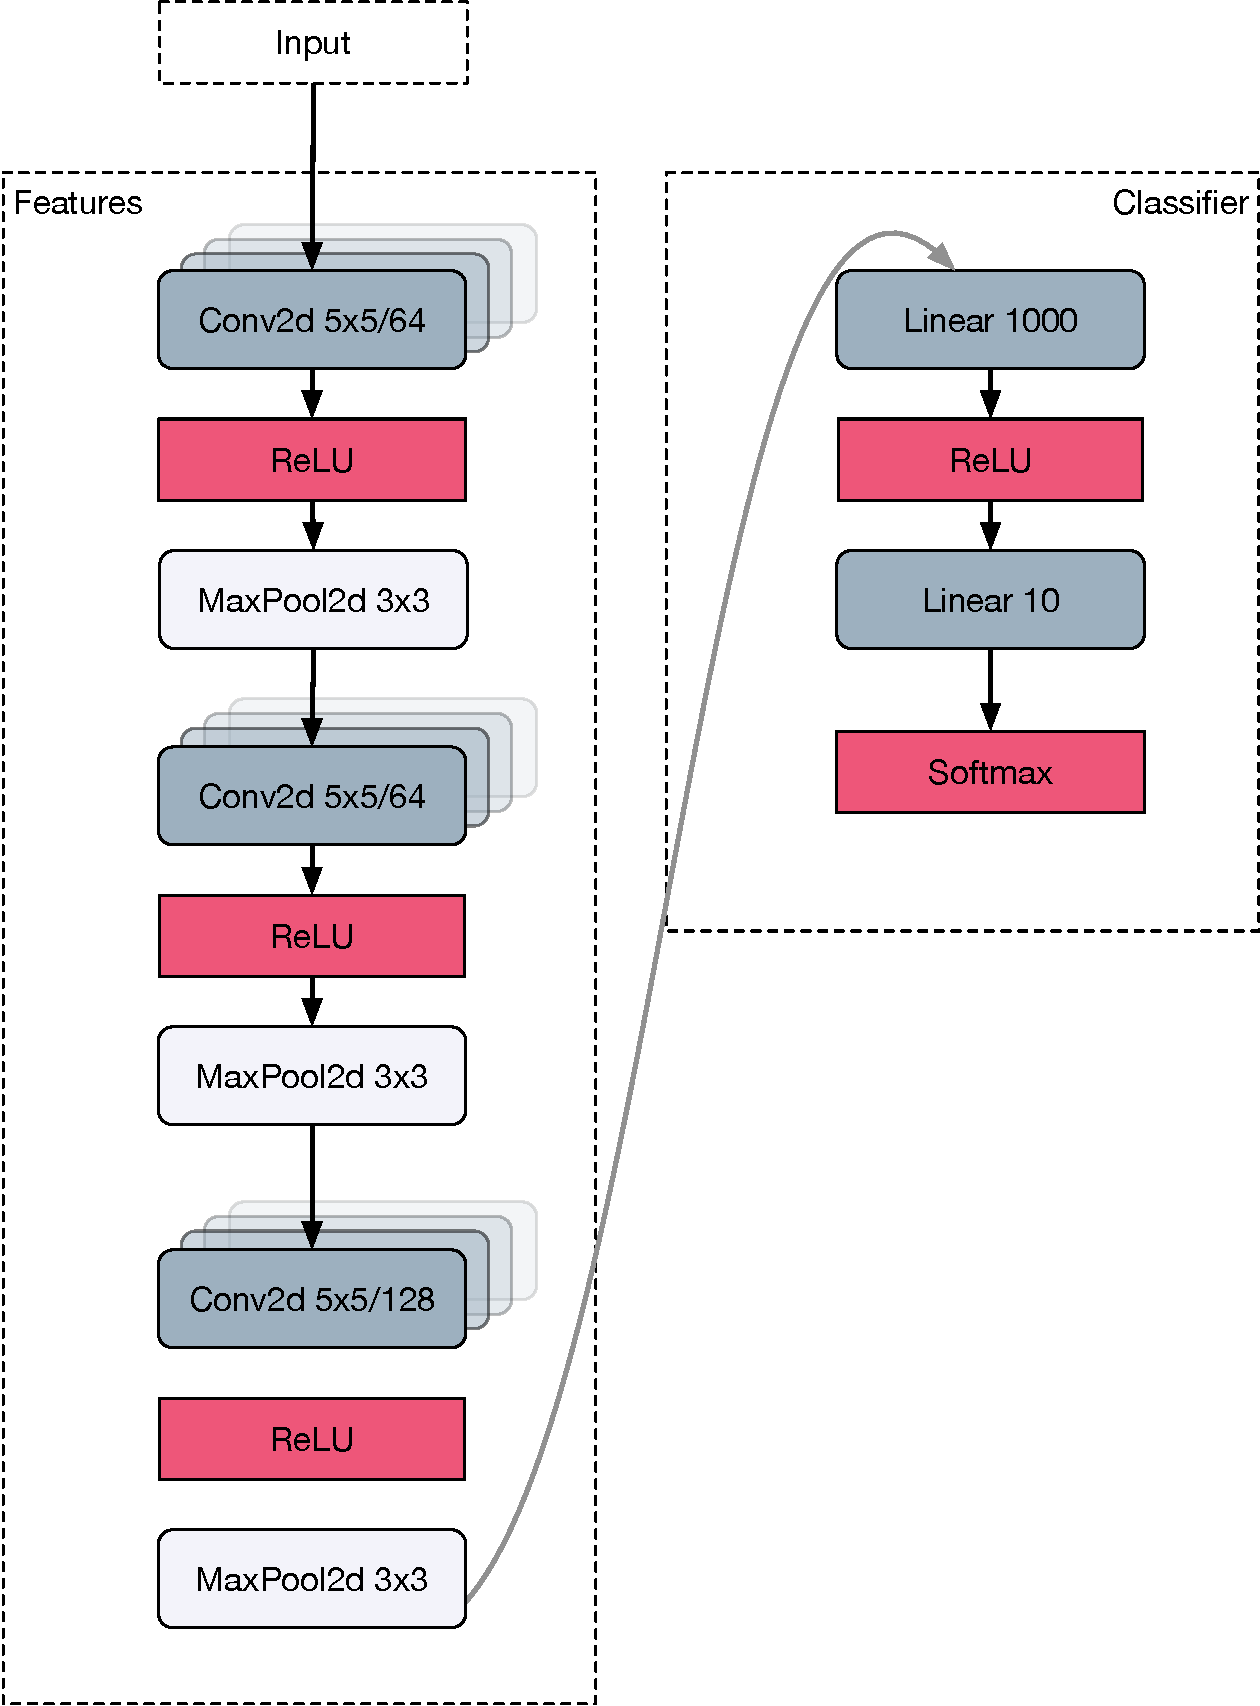
\includegraphics[width=\linewidth]{gfx/diagrams/neural_network/adammodel.pdf}
    \caption{Probable model architecture from \citep{kingma2014adam}}
    \label{fig:adammodel}
\end{figure}

\begin{figure}
    \centering
    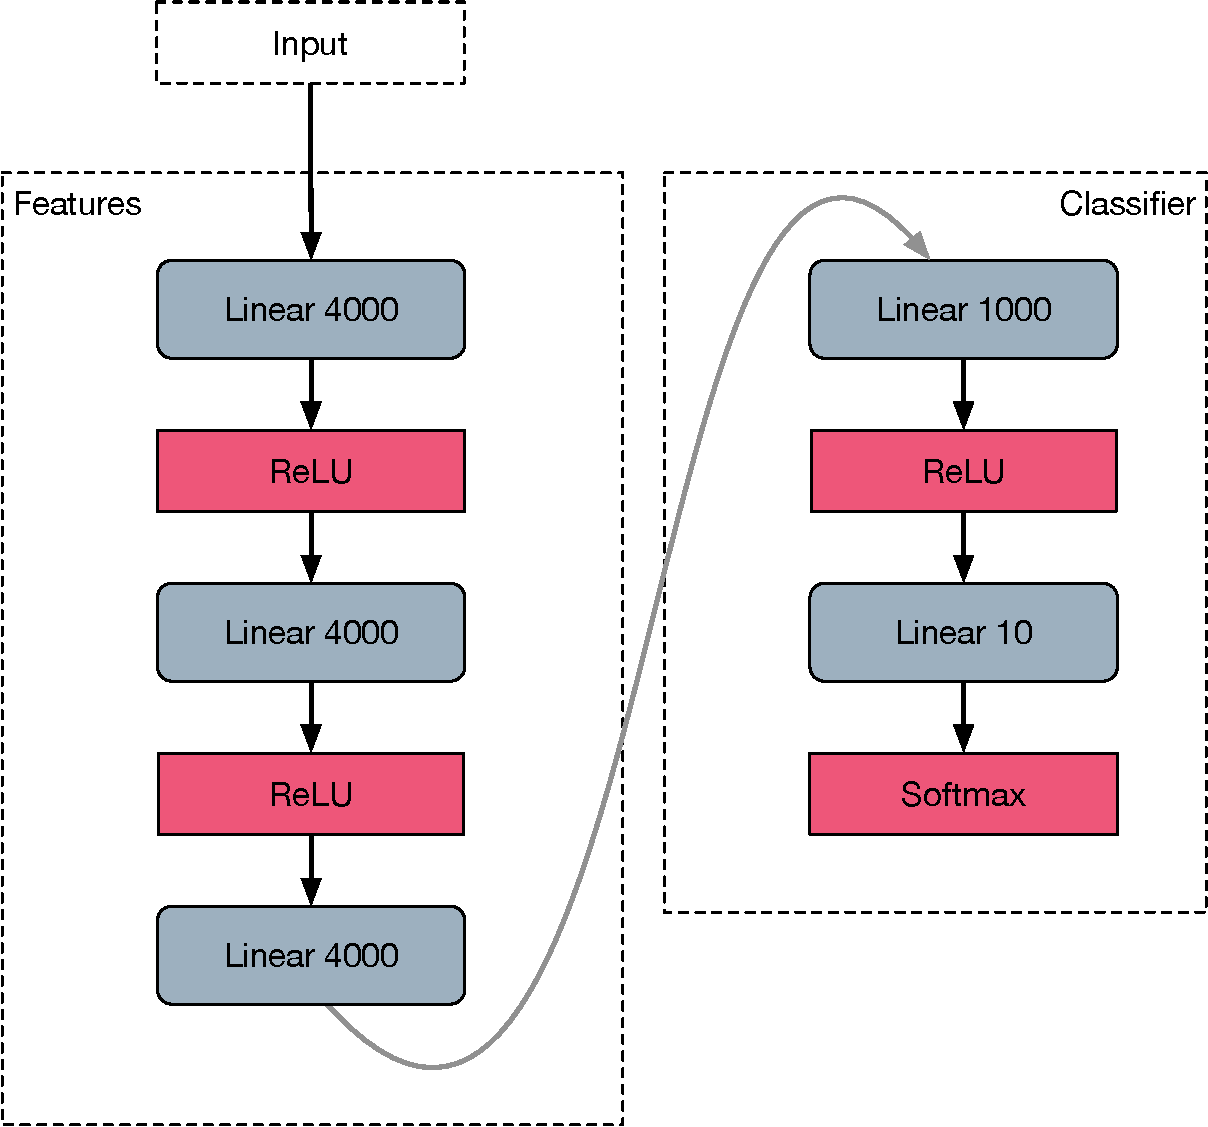
\includegraphics[width=\linewidth]{gfx/diagrams/neural_network/fullyconnected.pdf}
    \caption{Purely dense model}
    \label{fig:fully-connected}
\end{figure}

We want to employ \texttt{ikkuna} to monitor the quantities in Adam's update
rule on varous architectures. This will allow us to investigate whether there is
a qualitative difference in how Adam operates on different architectures, as
well as shed light on its behaviour in cases where it fails to optimise the
network. We also track the same quantites with vanilla SGD for comparison.
Additionally, the authors make claims in the publication without accompanying
evidence, notably

\begin{itemize}
    \item Convolutional layers should be assigned a smaller learning rate than
        linear ones and that -- presumably -- Adam does this automatically.
    \item
        That the update for the experiment with the convolutional network is
        dominated by the mean estimate and $\epsilon$ while the gradient
        variance estimate vanishes to zero after a few epochs.
\end{itemize}
Whether these assertions hold true will also be investigated.

It should be noted that the quantities used in \cref{eq:adam} are tensor-valued,
i.e. the estimates of the gradient moments are computed for each parameter.
Since visualising all parameters individually is not only computationally
infeasible, but also useless, some level of granularity with an appropriate
summary measure needs to be defined. The next level of organisation above
individual layer weights are the weight tensors themselves. Since layers are the
basic building blocks, it makes sense to investigate Adam's behaviour on the
level of individual layers. The question of how to summarise e.g. the gradient
mean estimate for an entire layer remains. Candidates are
\begin{enumerate}
    \item the average over all units
    \item the norm of the estimate
    \item the median over all units
\end{enumerate}
The first option suffers from the fact that the variance of the mean estimates
is (empirically) extremely high, so that the scalar summary will be dominated by
outliers, or be very close to zero as the magnitude of different dimensions
average out. The norm of the estimate of course suffers from the outlier problem
as well, but at least gives a sense of the total magnitude and thus the total
change to a layer. The last option is computationally more demanding, but
prevents the problem of outliers, while also suffering from the fact that the
gradient distribution is mostly centered around zero. However, we will first use
the median since it is an intuitive summary and the variance estimate and
effective learning rate do not have the zero-centeredness problem.

\subsubsection{Reproducing the Convnet experiment}

As a start, we check whether we can successfully recreate the experiment from
\citet{kingma2014adam} with the convolutional architecture. On p. 7 they show
the performance of the network over the first three epochs and the entire
training time. Our reproduction with the exact same parameters  is shown in
\cref{fig:adam-repro}.

\begin{figure}
    \begin{subfigure}{\textwidth}
        \centering
        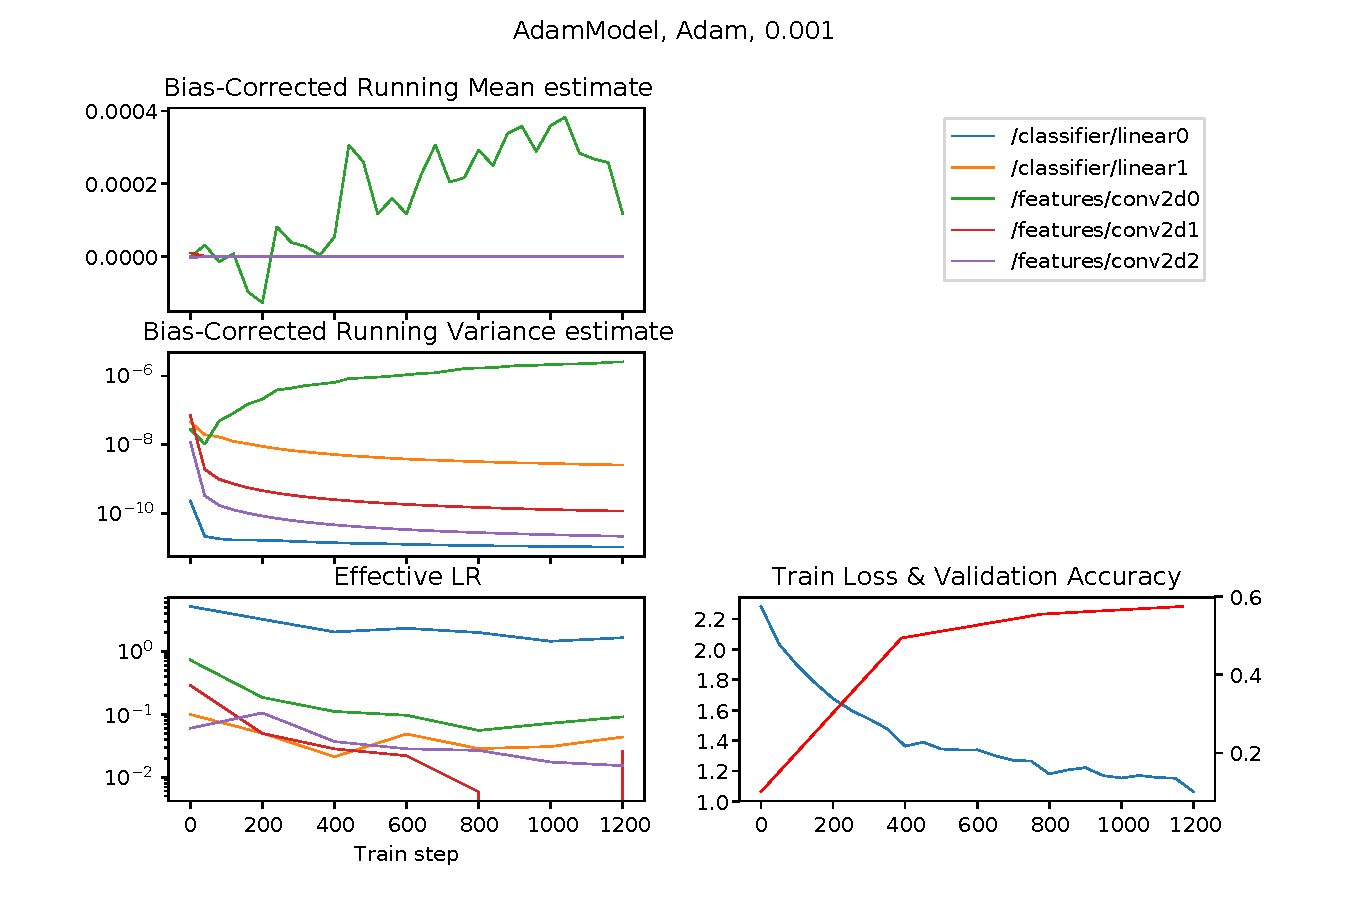
\includegraphics[width=\linewidth]{gfx/diagrams/experiments/adam/adammodel/adammodel_adam_0001_0_1200.pdf}
        \caption{Adam convnet with learning rate $0.0005$, first three epochs}
        \label{fig:adam-repro-1}
    \end{subfigure}

    \begin{subfigure}{\textwidth}
        \centering
        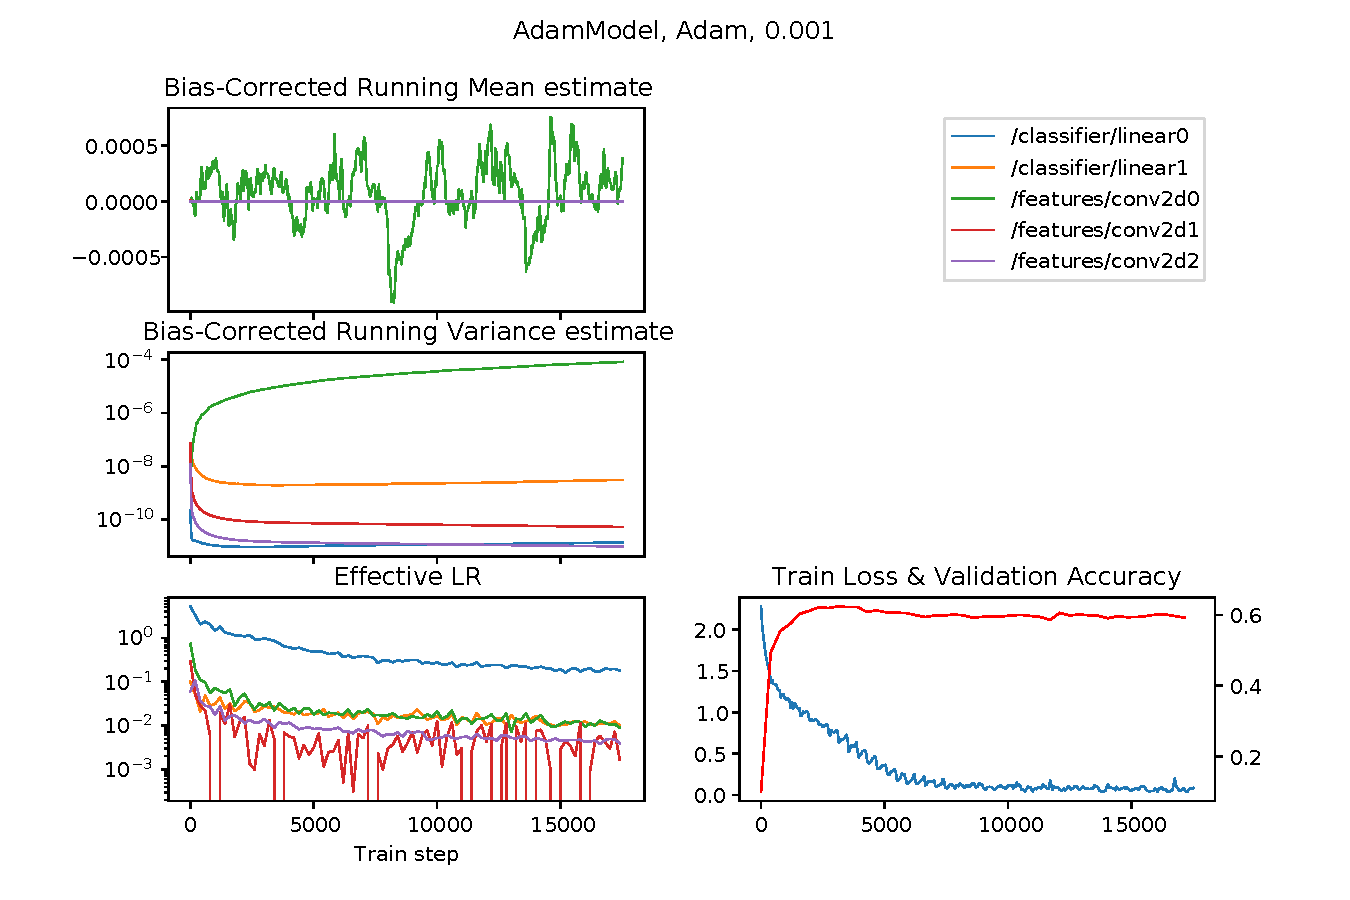
\includegraphics[width=\linewidth]{gfx/diagrams/experiments/adam/adammodel/adammodel_adam_0001_0_-1.pdf}
        \caption{Adam convnet with learning rate $0.001$, entire training}
        \label{fig:adam-repro-2}
    \end{subfigure}
    \label{fig:adam-repro}
\end{figure}

\citeauthor{kingma2014adam} report a decrease of the training cost from $\sim
2.2$ down to around $0.4$ over the course of the first three epochs. In our
reproduction (\cref{fig:adam-repro-1}), the loss does not decrease that rapidly,
but the trajectory is broadly similar, also when considering the entire training
(\cref{fig:adam-repro-2}). Nevertheless, the original setup achieves training
loss of less than $0.001$ while our experiment does not improve beypng $0.05$.
In \citeauthor{kingma2014adam}'s experiment, the
training loss almost saturates after about 20 epochs, the same holds for our
reproduction. However, the original result shows the network gradually learning
the entire time whereas performance basically stalls in our reproduction after
20 epochs. We can thus not completely reproduces the original experiment.
Possible reasons are an incorrectly specified architecture, or details of the
training procedure which \citeauthor{kingma2014adam} do not mention.
